\label{sec:metodologia}

\subsection{Especificaciones técnicas del proyecto}

Antes de pasar a explicar el código implementado, es importante mencionar las especificaciones técnicas del proyecto así como algunos requerimientos técnicos para tener un mejor entendimiento de los módulos implementados y su uso. 
\vspace{\baselineskip}

El proyecto se ha desarrollado en un entorno virtual, a través del software de virtualización \textit{Oracle VirtualBox}\footnote{https://www.virtualbox.org/}, en el cual se ha instalado el sistema operativo \textit{Xubuntu}\footnote{https://xubuntu.org/} que es una distribución Linux basada en Ubuntu (Ver Figura \ref{fig:oraclexubuntu}). El lenguaje de programación, usado ya en \textit{InterCom} y que se ha usado también para seguir desarrollándolo con los nuevos módulos implementados en este trabajo, es Python. 
\vspace{\baselineskip}

\begin{center}
	
\includegraphics[width = 0.32\textwidth]{images/oracle_xubuntu.png}
	\captionof{figure}{Logo de Oracle VirtualBox y Xubuntu.}
	\label{fig:oraclexubuntu}
\end{center}

\vspace{\baselineskip}

Para el correcto funcionamiento de \textit{InterCom} así como de los módulos desarrollados en este trabajo, hay que instalar diversos paquetes y hacer uso de bibliotecas concretas que se detallan a continuación. A continuación, se muestra en la Tabla \ref{tab:paquetes} la lista de paquetes y bibliotecas necesarias para el correcto funcionamiento del sistema \textit{InterCom} y de los módulos implementados en este trabajo.
\vspace{\baselineskip}

\begin{center}
\begin{tabular}{|p{2.5cm}|p{12.6cm}|}
    \hline
    \textbf{Paquete} & \textbf{Descripción } \\
    \hline
    argcomplete & Herramienta que proporciona el autocompletado en la linea de comandos, con la tecla TAB para aplicaciones Python que utilizan ``argparse''. \\
    \hline
    pywavelets & Biblioteca de Python para el análisis de señales y procesamiento de imágenes mediante transformadas wavelet (ondículas)~\cite{pywavelets}. \\
    \hline
    sounddevice & Biblioteca que permite grabar y reproducir audio en tiempo real a través de la tarjeta de sonido del sistema~\cite{sounddevice}. \\
    \hline
    soundfile & Lectura y escritura de la mayoría de formatos de archivo de sonido~\cite{soundfile}. \\
    \hline
    matplotlib & Creación de gráficos y visualizaciones estáticas/interactivas~\cite{matplotlib}. \\
    \hline
    scipy & Biblioteca fundamental para la computación científica y técnica~\cite{scipy}. \\
    \hline
    spectrum & Biblioteca que sirve para calcular y visualizar el espectro de frecuencias de una señal digital~\cite{spectrum}. \\
    \hline
    numpy & Soporte para arrays y matrices multidimensionales grandes. \\
    \hline
    psutil & Información del sistema y monitorización de procesos. \\
    \hline
    opencv-python & Biblioteca para la visualización del vídeo en tiempo real y visión artificial. \\
    \hline
    pygame & Conjunto de módulos Python para el desarrollo de videojuegos y aplicaciones multimedia. \\
    \hline
    pygame\_widgets & Proporciona widgets listos para usar en aplicaciones y juegos desarrollados con pygame~\cite{pygame_widgets}. \\
    \hline
    setuptools & Biblioteca y conjunto de herramientas para facilitar la creación, empaquetado, distribución e instalación de proyectos Python. \\
    \hline
\end{tabular}
\captionof{table}{Paquetes y bibliotecas utilizadas.}
\label{tab:paquetes}
\end{center}

\newpage

\subsection{Decisiones de diseño e implementación}

Para el desarrollo del sistema \textit{InterCom}, se han tomado diversas decisiones técnicas que, según los distintos requerimientos proporcionados por el tutor, deben tener los módulos haciendo que su funcionamiento y características sean concretas y diferentes a muchos otros programas de intercomunicación y que sea coherente con el sistema ya existente \textit{InterCom}. A continuación se detallan las más relevantes.

\subsubsection{Uso de UDP en lugar de TCP y sin compresión de vídeo}

Para la transmisión de vídeo y audio en tiempo real se ha optado por UDP (User Datagram Protocol) en vez de TCP (Transmission Control Protocol) por varias razones:

\begin{itemize} 
    \item \textbf{Latencia:} UDP no requiere establecimiento de conexión ni confirmación de recepción, lo que reduce significativamente la latencia en comparaciones con TCP~\cite{lpi}. 
    \item \textbf{Inmediatez:} El uso de UDP nos permite recibir el \texttt{frame} de vídeo más reciente aunque se pierdan algunos paquetes, en vez de esperar a reproducir paquetes antiguos que ya no serían relevantes~\cite{rfc768}. 
    \item \textbf{Eficiencia:} Al no tener sobrecarga por confirmaciones ni control de congestión, UDP aprovecha mejor el ancho de banda disponible en escenarios de comunicación en tiempo real~\cite{cloudflare_udp}. 
\end{itemize}

Además, en los módulos implementados en este trabajo, se ha mantenido la característica que ya implementaba \textit{InterCom} en sus módulos más basicos (\textit{Minimal} y \textit{Buffering}), que es la transmisión de los datos, solo de audio, sin usar ningún tipo de compresión de los mismos. Por lo tanto, para que se mantenga la coherencia con el sistema ya existente, en sus módulos básicos, se ha hecho lo mismo pero para los datos de vídeo. Sin embargo, como se puede ver en la Figura \ref{fig:jeraquia}, a partir del módulo \textit{DEFLATE}, se implementa la compresión de datos en el resto de módulos.

\subsubsection{Estructura de los paquetes de vídeo}

Cada paquete de vídeo enviado contiene:

\begin{itemize}
    \item \textbf{Cabecera (Header):} Un entero de 2 bytes (uint16) en formato big-endian que representa el índice del fragmento (FragIdx).
    \item \textbf{Carga útil (Payload):} Una porción de los datos de imagen sin comprimir (raw). \\
    Tiene un tamaño máximo de \texttt{effective\_video\_payload\_size - 2 bytes}.
\end{itemize}

\noindent
El paquete se construye así:
\begin{center}
\resizebox{0.95\textwidth}{!}{
\fbox{
    \texttt{[ FragIdx (2 bytes) ] [ Datos RAW de la imagen (hasta video\_payload\_size - 2 bytes) ]}
}
}
\end{center}

\subsubsection{Gestión de paquetes perdidos}

El sistema no implementa corrección de paquetes perdidos mediante retransmisiones por varias razones:

\begin{itemize}
    \item \textbf{Transmisión en tiempo real}: Se prioriza la continuidad del flujo sobre la integridad perfecta de cada fotograma.
    \item \textbf{Visualización}: La pérdida ocasional de fragmentos de vídeo es visualmente poco perceptible por lo que no nos importa que se pierdan algunos fragmentos.
    \item \textbf{Simplicidad}: Evita la complejidad adicional de buffers de reordenamiento y otros mecanismos de transmisión.
\end{itemize}

\subsubsection{Arquitectura de las clases principales y sus métodos}

La implementación se estructura en tres clases principales para mantener una separación clara de las distintas funcionalidades que realizan cada una de ellas:

\begin{itemize}
    \item \textbf{Minimal\_Video}: Clase base que extiende de \texttt{Minimal}, encargada de la funcionalidad principal de captura, transmisión, recepción y visualización del vídeo, manteniendo la compatibilidad con el sistema de audio existente en \textit{Minimal}.
    \item \textbf{Minimal\_Video\_FPS}: Clase que extiende de \textit{Minimal\_Video} y añade la funcionalidad de control de frames por segundo (FPS) para limitar la tasa de envío de fotogramas, permitiendo una mayor estabilidad en redes con limitaciones de ancho de banda. Se implementa el control de FPS en esta clase aparte debido a que OpenCV presenta problemas al establecer el FPS directamente en la cámara, lo que puede causar inestabilidad en la transmisión de vídeo. Por lo tanto, se ha optado por implementar un control de FPS a nivel de software, regulando la frecuencia de envío de fotogramas.
    \item \textbf{Minimal\_Video\_Resolution}: Clase que extiende de \textit{Minimal\_Video\_FPS} que permite ajustar y reescalar la resolución del vídeo, adaptándose a las capacidades del dispositivo de la cámara y a las preferencias del usuario.
\end{itemize}

Por ultimo, en la Figura \ref{fig:clases_methods_video} se muestra la jerarquía de clases y métodos implementados en todos los módulos desarrollados en este trabajo y una breve descripción de la funcionalidad de cada uno de los métodos.
\begin{center}
    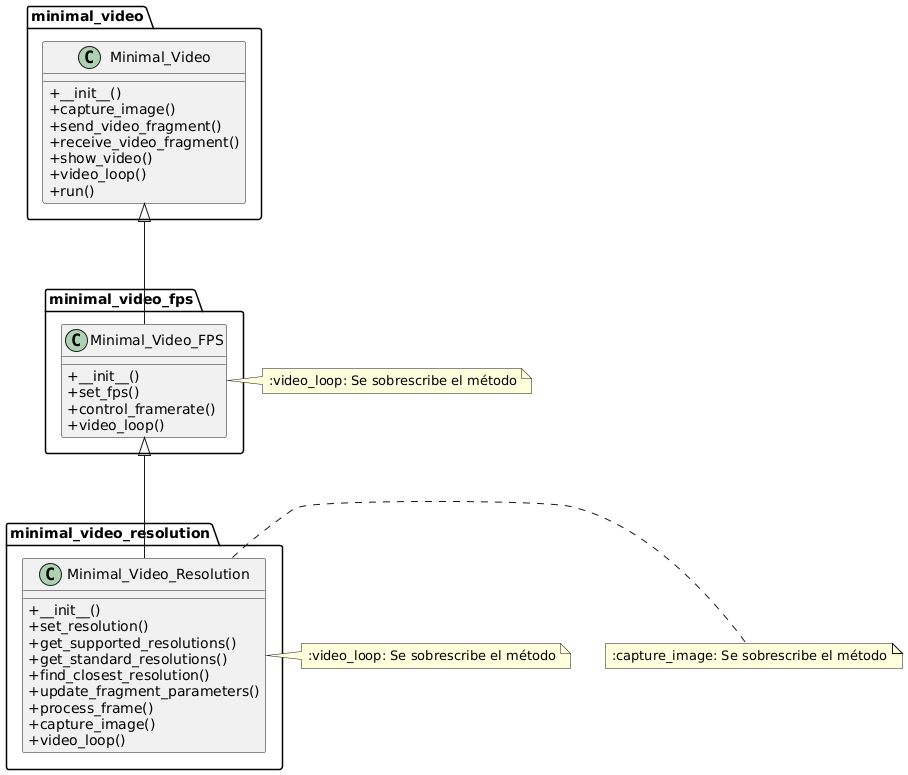
\includegraphics[width = 0.91\textwidth]{images/uml.png}
    \captionof{figure}{Jerarquía de clases y métodos implementados en los módulos de vídeo.}
    \label{fig:clases_methods_video}
\end{center}

La jerarquía de clases comienza con \texttt{Minimal\_Video} como la clase base para la comunicación de audio y vídeo, esta a su vez, extiende en dos clases adicionales para añadir funcionalidades específicas de vídeo:
\begin{itemize} 
    \item \texttt{Minimal\_Video} hereda de \texttt{Minimal} añadiendo funcionalidad de captura, envío, recepción y visualización de vídeo. 
    \item \texttt{Minimal\_Video\_FPS} hereda de \texttt{Minimal\_Video} añadiendo control de frames por segundo (FPS) para regular la tasa de envío de fotogramas.
    \item \texttt{Minimal\_Video\_Resolution} hereda de \texttt{Minimal\_Video\_FPS} añadiendo la capacidad de ajustar la resolución del vídeo teniendo en cuenta las resoluciones permitidas por la cámara y realizar, si fuera necesario, su reescalado a la nueva resolución.
\end{itemize}

Ahora, se detallarán los métodos de las clases desarrolladas en este trabajo:
\vspace{\baselineskip}

\textbf{· Métodos de Minimal\_Video:} 
\begin{itemize} 
    \item \texttt{\_\_init\_\_()}: Inicializa configuración de vídeo y socket UDP para comunicación. 
    \item \texttt{capture\_image()}: Captura un fotograma desde la cámara y lo devuelve como bytes. 
    \item \texttt{send\_video\_fragment()}: Envía un fragmento del fotograma con su cabecera por UDP. 
    \item \texttt{receive\_video\_fragment()}: Recibe un fragmento y lo coloca en la posición correcta del frame remoto. 
    \item \texttt{show\_video()}: Muestra el fotograma recibido en una ventana usando OpenCV. 
    \item \texttt{video\_loop()}: Gestiona el ciclo continuo de captura, envío, recepción y visualización. 
    \item \texttt{run()}: Inicia un hilo para el bucle de vídeo y ejecuta la funcionalidad de audio heredada. 
\end{itemize}

\textbf{· Métodos de Minimal\_Video\_FPS:} 
\begin{itemize} 
    \item \texttt{\_\_init\_\_()}: Extiende la inicialización de \texttt{Minimal\_Video} para incluir configuración de FPS. 
    \item \texttt{set\_fps()}: Establece el FPS objetivo basado en los argumentos de entrada. 
    \item \texttt{control\_framerate()}: Controla la tasa de fotogramas para cumplir con el FPS objetivo.
    \item \texttt{video\_loop()}: Sobrescribe el bucle para añadir el control de FPS al ciclo de vídeo. 
\end{itemize}

\textbf{· Métodos de Minimal\_Video\_Resolution:} 
\begin{itemize} 
    \item \texttt{\_\_init\_\_()}: Extiende la inicialización de \texttt{Minimal\_Video\_FPS} para incluir configuración de resolución. 
    \item \texttt{set\_resolution()}: Establece la resolución objetivo desde los parámetros. 
    \item \texttt{get\_supported\_resolutions()}: Obtiene las resoluciones compatibles con la cámara. 
    \item \texttt{get\_standard\_resolutions()}: Proporciona una lista de resoluciones estándar cuando no se detectan específicas. 
    \item \texttt{find\_closest\_resolution()}: Busca la resolución disponible más cercana a la solicitada. 
    \item \texttt{update\_fragment\_parameters()}: Recalcula parámetros de fragmentación para la nueva resolución. 
    \item \texttt{process\_frame()}: Redimensiona el fotograma si es necesario. 
    \item \texttt{capture\_image()}: Sobrescribe para incluir procesamiento de resolución. 
    \item \texttt{video\_loop()}: Sobrescribe el bucle de vídeo para incluir el procesamiento de resolución.
\end{itemize}

\newpage

\subsection{Código implementado}
En esta sección, se procederá a comentar, prácticamente, línea por línea o en su defecto bloques de código similares, para mayor entendimiento del mismo. A su vez, cada módulo se dividirá en dos subsecciones para explicar tanto la versión normal del código como la ``verbose''. El código completo implementado en este trabajo se encuentra disponible en el repositorio de GitHub \url{https://github.com/JJsanriv/TFG-Intercom-Video}.

\subsubsection{Código del módulo Minimal\_Video}

En primer lugar, se comenzará por explicar el código del módulo \textit{Minimal\_Video} que es el módulo base que se encarga de la captura, transmisión, recepción y visualización del vídeo. Los otros dos módulos que se han desarrollado en este trabajo parten de este, por lo que, muchos métodos y la estructura son muy similares y se sigue la misma lógica en todos ellos. El código de este módulo es el siguiente:
\begin{lstlisting}[style=pythonstyle, caption={Comienzo del módulo \textit{Minimal\_Video} y sus parámetros.}, label={lst:principio_clase_minimal}]
#!/usr/bin/env python
# PYTHON_ARGCOMPLETE_OK

import cv2
import socket
import struct
import threading
import time
import math
import numpy as np
import select
import argparse
import psutil
import minimal

spinner = minimal.spinning_cursor()

def int_or_str(text):
    try:
        return int(text)
    except ValueError:
        return text

if not hasattr(minimal, 'parser'):
    minimal.parser = argparse.ArgumentParser(formatter_class=argparse.ArgumentDefaultsHelpFormatter)
parser = minimal.parser

parser.add_argument("-v", "--video_payload_size", type=int, default=1400, help="Desired size (bytes) of video payload/UDP fragment (default 1400).")
parser.add_argument("-w", "--width", type=int, default=320, help="Video width (default 320)")
parser.add_argument("-g", "--height", type=int, default=240, help="Video height (default 240)")
parser.add_argument("-z", "--fps", type=int, default=30, help="Video frames per second (default 30)")
parser.add_argument("--show_video", action="store_true", default=False, help="Enables video visualization and transmission (disabled by default).")
parser.add_argument("-lvp", "--listening_video_port", type=int, default=4445, help="Port to listen on for receiving video (default 4445).")
parser.add_argument("-dvp", "--destination_video_port", type=int, default=4445, help="Port to send video to (default 4445).")
parser.add_argument("--camera_index", type=int, default=0, help="Index of the camera to use (default 0).")

args = None
\end{lstlisting}

A continuación, se encuentra la explicación del código mostrado en el Listado \ref{lst:principio_clase_minimal}:

\begin{itemize}
    \item \textbf{Línea 1:} se define el ``shebang'' que indica que el script debe ejecutarse con Python.
    \item \textbf{Línea 2:} se indica que el script es compatible con la autocompletación de argumentos en la línea de comandos.
    \item \textbf{Líneas 4-14:} se importan las bibliotecas necesarias para el funcionamiento del módulo. Estas bibliotecas son fundamentales para la captura, transmisión y recepción de vídeo, así como para la manipulación de datos y la creación de sockets.
    \item \textbf{Línea 16:} se define el objeto \texttt{spinner} que se usará para mostrar un cursor giratorio en la línea de comandos mientras se espera la entrada del usuario.
    \item \textbf{Líneas 18-22:} se define la función \texttt{int\_or\_str()} que intenta convertir un texto en un entero. Si no puede, devuelve el texto original. Esta función se usará para procesar argumentos de línea de comandos.
    \item \textbf{Líneas 24-26:} se verifica si el módulo \textit{Minimal} tiene un atributo llamado \texttt{parser}. Si no lo tiene, se crea un nuevo objeto \texttt{ArgumentParser} para procesar los argumentos de línea de comandos. Este objeto se usará para definir y gestionar los argumentos que se pasan al script.
    \item \textbf{Línea 28-35:} se definen varios argumentos de línea de comandos que se pueden usar al ejecutar el script. Estos argumentos permiten al usuario personalizar el comportamiento del módulo, como el tamaño del payload de vídeo, las dimensiones del vídeo, los frames por segundo, la habilitación de la visualización del vídeo y los puertos de escucha y destino para la transmisión de vídeo así como el índice que usa la cámara. Cada argumento tiene un tipo, un valor por defecto y una descripción.
    \item \textbf{Línea 37:} se inicializa la variable \texttt{args} como \texttt{None}. Esta variable se usará para almacenar los argumentos procesados por el parser.
\end{itemize}

\vspace{\baselineskip}

Ahora, se procede a explicar el comienzo de la clase \textit{Minimal\_Video} y parte del método \texttt{\_init\_} que es el que se encarga de inicializar la clase y sus atributos. El código es el siguiente:

\begin{lstlisting}[style=pythonstyle, caption={Comienzo de la clase \textit{Minimal\_Video} y parte de la inicialización.}, label={lst:inicializacion_minimal_video}]
class Minimal_Video(minimal.Minimal):
    def __init__(self):
        global args
        if args is None:
            args = minimal.parser.parse_args()
        minimal.args = args

        super().__init__()

        if not args.show_video:
            return

        self.video_sock = socket.socket(socket.AF_INET, socket.SOCK_DGRAM)
        self.video_sock.setsockopt(socket.SOL_SOCKET, socket.SO_REUSEADDR, 1)
        self.video_sock.setsockopt(socket.SOL_SOCKET, socket.SO_RCVBUF, 8388608)
        self.video_sock.setsockopt(socket.SOL_SOCKET, socket.SO_SNDBUF, 8388608)
        self.video_sock.setblocking(False)
        try:
            self.video_sock.bind(("0.0.0.0", args.listening_video_port))
        except OSError as e:
            print(f"Error binding video socket: {e}")
            raise
        self.video_addr = (args.destination_address, args.destination_video_port)

        self._header_format = "!H"
        self.header_size = 2
        self.effective_video_payload_size = args.video_payload_size
        self.max_payload_possible = self.effective_video_payload_size - self.header_size
        self.effective_video_payload_size = max(1, min(args.video_payload_size, self.max_payload_possible))
        if self.effective_video_payload_size != args.video_payload_size:
            print(f"Warning: --video_payload_size adjusted to {self.effective_video_payload_size} bytes.")

        self.cap = None
        self.width = 0
        self.height = 0
        self.fps = 0

        self.expected_frame_size = 0
        self.total_frags = 0
\end{lstlisting}

A continuación, se encuentra la explicación del código mostrado en el Listado \ref{lst:inicializacion_minimal_video}:

\begin{itemize}
    \item \textbf{Línea 1:} se define la clase \textit{Minimal\_Video} que hereda de la clase \textit{Minimal} del módulo \textit{Minimal}.
    \item \textbf{Línea 2:} se define el método \texttt{\_\_init\_\_} que es el constructor de la clase.
    \item \textbf{Líneas 3-6:} se inicializa la variable \texttt{args} con los argumentos procesados por el parser. Si \texttt{args} ya tiene un valor, se omite esta parte.
    \item \textbf{Línea 8:} se llama al constructor de la clase padre \textit{Minimal} para inicializar sus atributos.
    \item \textbf{Líneas 10-11:} se verifica si la opción de mostrar vídeo está habilitada. Si no lo está, se sale del método ya que no necesitaríamos inicializar todas las variables y métodos correspondientes con el vídeo.
    \item \textbf{Línea 13:} se crea un socket UDP para la transmisión de vídeo. socket.AF\_INET indica que se usará IPv4 y socket.SOCK\_DGRAM indica que se usará UDP.
    \item \textbf{Líneas 14-16:} se configuran opciones del socket para permitir la reutilización de la dirección IP y puertos usados\footnote{La reutilización de la dirección sirve para que no nos muestre el error ``Address already in use'' al ejecutar el módulo varias veces seguidas.} y aumentar el tamaño del buffer de recepción y envío a 8MB\footnote{Permite mayor flexibilidad al manejar mayor cantidad de datos de vídeo sin pérdidas cuando hay picos en la recepción.}.
    \item \textbf{Línea 17:} se establece el socket como no bloqueante, lo que significa que las operaciones de lectura y escritura no bloquearán el socket de vídeo si no hay datos disponibles.\footnote{Permite que el módulo continúe ejecutándose mientras maneja la comunicación de vídeo sin quedar bloqueado. Esencial para aplicaciones en tiempo real, en concreto la nuestra.}
    \item \textbf{Líneas 18-22:} se configura el socket para escuchar conexiones entrantes en todas las interfaces de red (dirección IP ``0.0.0.0'') en el puerto especificado por el argumento listening\_video\_port.\footnote{ Si la operación falla (por ejemplo, porque el puerto ya está en uso), captura el error OSError, muestra un mensaje descriptivo y lanza la excepción para terminar la ejecución del módulo.}
    \item \textbf{Línea 23:} se inicializa la variable \texttt{video\_addr} con la dirección IP de destino y el puerto de vídeo de destino.
    \item \textbf{Línea 25-26:} se define el formato del encabezado del paquete de vídeo como un entero sin signo de 16 bits (2 bytes) usando el formato de la biblioteca struct. 
    \item \textbf{Líneas 27-31:} Primero asigna el valor proporcionado por el usuario \texttt{args.video\_payload\_size} a \texttt{self.effective\_video\_payload\_size}. Luego, se calcula el máximo payload posible restando el tamaño de la cabecera (\texttt{self.header\_size}) del tamaño deseado. \\
    \texttt{self.effective\_video\_payload\_size} se ajusta para que esté entre 1 y el máximo payload posible calculado. Por ultimo, si el valor final es diferente del solicitado por el usuario, muestra un mensaje de aviso indicando que se ha ajustado automáticamente.\footnote{Este trozo de código garantiza que el tamaño del payload sea válido para la transmisión de vídeo, evitando valores demasiado pequeños o muy grandes que superen el límite permitido por el tamaño de la cabecera.}
    \item \textbf{Líneas 33-36:} se inicializan varias variables relacionadas con la captura de vídeo. \texttt{self.cap} se usará para almacenar el objeto de captura de vídeo, \texttt{self.width} y \texttt{self.height} almacenan las dimensiones del vídeo, \texttt{self.fps} almacena los frames por segundo.
    \item \textbf{Líneas 38-39:} se inicializan las variables \texttt{self.expected\_frame\_size} y \texttt{self.total\_frags} que se usarán para almacenar el tamaño esperado de un fotograma y el número total de fragmentos del vídeo.
\end{itemize}

\vspace{\baselineskip}

Terminamos la función \texttt{\_init\_} de la forma que se observa en el código mostrado en el Listado \ref{lst:fin_ini_minimal_video}.
\vspace{\baselineskip}
\begin{lstlisting}[style=pythonstyle, caption={Fin de la inicialización de \textit{Minimal\_Video}.}, label={lst:fin_ini_minimal_video}]
print(f"Flag --show_video detected. Attempting to initialize camera with index {args.camera_index}...")
        try:
            self.cap = cv2.VideoCapture(args.camera_index)
            if not self.cap.isOpened():
                raise IOError(f"Could not open camera with index {args.camera_index}.")
            if args.width > 0:
                self.cap.set(cv2.CAP_PROP_FRAME_WIDTH, args.width)
            if args.height > 0:
                self.cap.set(cv2.CAP_PROP_FRAME_HEIGHT, args.height)
            if args.fps > 0:
                self.cap.set(cv2.CAP_PROP_FPS, args.fps)
            self.cap.set(cv2.CAP_PROP_BUFFERSIZE, 2)
            self.width = int(self.cap.get(cv2.CAP_PROP_FRAME_WIDTH))
            self.height = int(self.cap.get(cv2.CAP_PROP_FRAME_HEIGHT))
            self.fps = int(self.cap.get(cv2.CAP_PROP_FPS))

            self.expected_frame_size = self.width * self.height * 3
            self.total_frags = math.ceil(self.expected_frame_size / self.effective_video_payload_size)

            self.fragment_ranges = []
            self.fragment_headers = []
            for frag_idx in range(self.total_frags):
                start = frag_idx * self.effective_video_payload_size
                end = min(start + self.effective_video_payload_size, self.expected_frame_size)
                self.fragment_ranges.append((start, end))
                self.fragment_headers.append(struct.pack(self._header_format, frag_idx))

            self.remote_frame = np.zeros((self.height, self.width, 3), dtype=np.uint8)
            
        except Exception as e:
            print(f"Error initializing camera: {e}. Disabling video.")
            if self.cap:
                self.cap.release()
            self.cap = None

        self.running = True
\end{lstlisting}

\begin{itemize}
    \item \textbf{Línea 1:} se imprime un mensaje indicando que se ha detectado la opción \verb|--show_video| y que se intentará inicializar la cámara con el indice de la misma.\footnote{Evidentemente el usuario tiene que tener la cámara conectada y activada.}
    \item \textbf{Líneas 2-5:} se intenta inicializar la cámara usando la función de OpenCV \texttt{VideoCapture()} con el índice de la cámara proporcionado por el usuario. Si no se puede abrir la cámara, se lanza una excepción \texttt{IOError} y se imprime un mensaje de error. Esto garantiza que el módulo no intente usar la cámara si no está disponible.
    \item \textbf{Líneas 6-11:} se configuran las propiedades de la cámara (ancho, alto y FPS) según los argumentos proporcionados por el usuario. Si los valores son mayores que 0, se aplican.
    \item \textbf{Línea 12:} se establece el tamaño del buffer de la cámara a 2 fotogramas\footnote{El tamaño del buffer se refiere a la cantidad de fotogramas que se almacenan temporalmente antes de ser procesados. Se usa un buffer de 2 fotogramas en lugar de 1 porque muchos drivers de cámara no funcionan correctamente con un buffer de solo 1 frame, pudiendo causar errores, frames corruptos o comportamiento inestable. El uso de 2 fotogramas es el mínimo que garantiza estabilidad del sistema mientras mantiene una latencia muy baja, proporcionando un pequeño margen de seguridad contra \textit{frame drops} sin sacrificar significativamente el rendimiento en tiempo real.}, lo que ayuda a reducir la latencia en la captura de vídeo.
    \item \textbf{Líneas 13-15:} se obtienen las dimensiones del vídeo (ancho, alto y FPS) y se almacenan en las variables correspondientes.
    \item \textbf{Líneas 17-18:} se calcula el tamaño esperado de un fotograma (en bytes) multiplicando el ancho, la altura y 3 (3 bytes por píxel para un vídeo RGB) y se almacena en \texttt{self.expected\_frame\_size}. Luego, se calcula el número total de fragmentos necesarios para enviar el fotograma completo dividiendo el tamaño esperado por el tamaño efectivo del payload de vídeo.
    \item \textbf{Líneas 20-21:} se inicializan dos listas \texttt{self.fragment\_ranges} y \texttt{self.fragment\_headers}. Estas listas se usarán para almacenar los rangos de fragmentos y los encabezados de cada fragmento.
    \item \textbf{Líneas 22-26:} se itera sobre el número total de fragmentos y se calcula el rango de bytes para cada fragmento. Se empaqueta el índice del fragmento en un encabezado usando \texttt{struct.pack} y se añaden a las listas correspondientes. Esto sirve para dividir el fotograma en fragmentos que se enviarán por separado a través de la red.
    \item \textbf{Línea 28:} esta línea crea un \texttt{frame} inicializado en negro (todos los valores en 0) para que sea el primer frame que se muestre y a partir de ahí que se actualicen con los frames reales.
    \item \textbf{Líneas 30-34:} este bloque de código garantiza que si ocurre un error al inicializar la cámara, se capture la excepción y se liberen los recursos utilizados así, el módulo puede continuar ejecutándose sin intentar usar el vídeo. Es una medida de seguridad y limpieza de recursos contra posible fallos del módulo.
    \item \textbf{Línea 36:} esta variable indica cuando la instancia de la clase está en ejecución y permite controlar el ciclo principal del procesamiento de vídeo y su transmisión. Cuando se termina la ejecución del módulo, se establece a ``false'' para que paren todos los procesos relacionados con el vídeo.
\end{itemize}

Ahora, una vez terminada la inicialización de la clase \textit{Minimal\_Video}, procedemos a explicar cada método que se usa para la captura, transmisión, recepción y captura de vídeo así como el método para ejecutar de forma correcta y adecuada estos mismos.
\vspace{\baselineskip}

Comenzamos con el método \texttt{capture\_image()} que se puede observar en el código mostrado en el Listado \ref{lst:capture_frame}, el cual realiza la captura de vídeo:
\begin{lstlisting}[style=pythonstyle, caption={Método \texttt{capture\_frame()} de \textit{Minimal\_Video}.}, label={lst:capture_frame}]
def capture_image(self):
        _, frame = self.cap.read()
        return frame.tobytes()
\end{lstlisting}

\begin{itemize}
    \item \textbf{Línea 1:} se define el método \texttt{capture\_image()} que no toma argumentos.
    \item \textbf{Línea 2:} se usa el método \texttt{read()} de OpenCV para capturar un fotograma de vídeo. Este método devuelve dos valores: \texttt{ret} un valor booleano que indica si la captura fue exitosa (usamos ``\_'' ya que no lo necesitamos) y \texttt{frame} (el fotograma capturado).
    \item \textbf{Línea 3:} si la captura es correcta, se convierte el fotograma a bytes usando el método \texttt{tobytes()} y se devuelve. Este método convierte la imagen capturada en un formato de bytes que se puede enviar a través de la red.
\end{itemize}
\vspace{\baselineskip}

El código mostrado en el Listado \ref{lst:send_fragment} se encargará de enviar los fragmentos de vídeo a través del socket de vídeo UDP:
\begin{lstlisting}[style=pythonstyle, caption={Método \texttt{send\_video\_fragment()} de \textit{Minimal\_Video}.}, label={lst:send_fragment}]
def send_video_fragment(self, frag_idx, data):
    start, end = self.fragment_ranges[frag_idx]
    payload = data[start:end]
    packet = self.fragment_headers[frag_idx] + payload
    try:
        self.video_sock.sendto(packet, self.video_addr)
    except BlockingIOError:
        print(f"Socket blocked while sending fragment {frag_idx}.")
        pass
    return len(packet)
\end{lstlisting}

\begin{itemize}
    \item \textbf{Línea 1:} se define el método \texttt{send\_video\_fragment} que toma como argumentos el índice del fragmento (\texttt{frag\_idx}) y los datos del fotograma (\texttt{data}).
    \item \textbf{Línea 2:} se obtienen los rangos de inicio y fin del fragmento correspondiente al índice proporcionado.
    \item \textbf{Línea 3:} se extraen los datos del fotograma en el rango especificado y se almacenan en la variable \texttt{payload}.
    \item \textbf{Línea 4:} se crea el paquete concatenando el encabezado del fragmento y los datos del fotograma.
    \item \textbf{Líneas 5-9:} se intenta enviar el paquete a través del socket de vídeo UDP usando el método \texttt{sendto()}. Si el socket está bloqueado, se captura la excepción \texttt{BlockingIOError} y se imprime un mensaje de advertencia. En este caso, simplemente se ignora.\footnote{Aunque el socket se estableció como no bloqueante, puede haber ocasiones en las que el socket esté temporalmente bloqueado debido a la congestión de la red o a otros factores.}
    \item \textbf{Línea 10:} se devuelve la longitud del paquete enviado, que será útil en módulos derivados de este.\footnote{Se verá más adelante en el módulo \textit{Minimal\_Video\_FPS} que se usa para calcular el tamaño del paquete enviado.}
\end{itemize}
\vspace{\baselineskip}

El código mostrado en el Listado \ref{lst:receive_fragment} se encuentra el método que se encarga de recibir los fragmentos de vídeo a través del socket de vídeo UDP:
\begin{lstlisting}[style=pythonstyle, caption={Método \texttt{receive\_video\_fragment()} de \textit{Minimal\_Video}.}, label={lst:receive_fragment}]
def receive_video_fragment(self):
        rlist, _, _ = select.select([self.video_sock], [], [], 0.001)
        if rlist:
            packet, addr = self.video_sock.recvfrom(self.effective_video_payload_size + self.header_size)
            header = packet[:self.header_size]
            payload = packet[self.header_size:]
            recv_frag_idx, = struct.unpack(self._header_format, header)
            start = recv_frag_idx * self.effective_video_payload_size
            end = min(start + len(payload), self.expected_frame_size)
            flat_frame = self.remote_frame.reshape(-1) # Flatten the frame for direct assignment
            flat_frame[start:end] = np.frombuffer(payload, dtype=np.uint8, count=(end - start)) # Direct assignment
            return recv_frag_idx, len(packet)
        return None, 0
\end{lstlisting}

A continuación, se explican las líneas de código que se muestran en el código mostrado en el Listado \ref{lst:receive_fragment}:
\begin{itemize}
    \item \textbf{Línea 1:} se define el método \texttt{receive\_video\_fragment} que no toma argumentos.
    \item \textbf{Línea 2:} se usa la función \texttt{select.select()} para esperar a que haya datos disponibles en el socket de vídeo. Esta función permite ver cuando el socket de vídeo esta libre para recibir el fragmento. En este caso, se espera un máximo de 1 milisegundos.\footnote{Ajustar el tiempo de espera a 1 ms ha sido la configuración más óptima encontrada.}
    \item \textbf{Línea 3:} si hay datos disponibles (\texttt{rlist} no está vacío), se entra en la condición.
    \item \textbf{Línea 4:} se recibe el paquete de datos del socket usando el método \texttt{recvfrom()}\footnote{El método \texttt{recvfrom} internamente realiza las siguientes operaciones: bloquea la ejecución hasta recibir datos en el socket de vídeo UDP, captura los bytes entrantes según el tamaño especificado (effective\_video\_payload\_size + header\_size), identifica la dirección IP y puerto del remitente, y devuelve tanto los datos recibidos como la información del remitente como una tupla (paquete, dirección).}. Este método devuelve el paquete recibido y la dirección del remitente. El tamaño máximo del paquete es el tamaño efectivo del payload más el tamaño del encabezado.
    \item \textbf{Línea 5:} se extrae el encabezado del paquete recibido.
    \item \textbf{Líneas 6:} se extraen los datos del payload del paquete recibido, omitiendo el encabezado.
    \item \textbf{Línea 7:} se desempaqueta el encabezado para obtener el índice del fragmento recibido usando la función \texttt{struct.unpack()}.\footnote{La función \texttt{struct.unpack()} convierte los bytes del encabezado en un entero, que representa el índice del fragmento recibido.}
    \item \textbf{Línea 8:} se define la variable \texttt{start} que representa el inicio del rango de bytes del fragmento recibido.
    \item \textbf{Línea 9:} se define la variable \texttt{end} que representa el final del rango de bytes del fragmento recibido.
    \item \textbf{Línea 10:} se aplana el fotograma remoto para facilitar la asignación directa de los datos del payload. Esto convierte el fotograma en un array unidimensional, lo que permite acceder a los elementos de manera más sencilla.\footnote{El método \texttt{reshape(-1)} convierte el array multidimensional en un array unidimensional, manteniendo el mismo número total de elementos.}
    \item \textbf{Línea 11:} se asignan directamente los datos del payload al rango correspondiente en el fotograma remoto usando la función \texttt{np.frombuffer()} para convertir los bytes en un array NumPy~\cite{numpy}. Esto permite que los datos del payload se copien directamente en el fotograma remoto en la posición correcta.\footnote{La función \texttt{np.frombuffer()} crea un array NumPy a partir de un buffer de bytes, permitiendo especificar el tipo de dato y la cantidad de elementos a leer.}
    \item \textbf{Línea 12:} se devuelve el índice del fragmento recibido y la longitud del paquete recibido.
    \item \textbf{Línea 13:} si no hay datos disponibles, se devuelve \texttt{None} y 0.
\end{itemize}
\vspace{\baselineskip}

Seguidamente, continuamos explicando el método \texttt{show\_video()} que es el que se encargará de mostrar el vídeo en una ventana utilizando \textit{OpenCV}:
\begin{lstlisting}[style=pythonstyle, caption={Método \texttt{show\_video()} de \textit{Minimal\_Video}.}, label={lst:show_video}]
    def show_video(self):
        cv2.imshow("Video (Cam {args.camera_index})", self.remote_frame)
        cv2.waitKey(1)
\end{lstlisting}

A continuación, se explican las líneas de código referentes al código mostrado en el Listado \ref{lst:show_video}:
\begin{itemize}
    \item \textbf{Línea 1:} se define el método \texttt{show\_video()} que no toma argumentos.
    \item \textbf{Línea 2:} se muestra el fotograma remoto en una ventana llamada ``Vídeo'' usando la función \texttt{cv2.imshow()} de OpenCV.
    \item \textbf{Línea 3:} se espera 1 milisegundo para permitir que la ventana se actualice y procese posibles pulsaciones del teclado usando la función \texttt{cv2.waitKey()}.
\end{itemize}
\vspace{\baselineskip}

El siguiente método \texttt{video\_loop()} es el más importante de la clase ya que es el bucle principal que captura, envía y recibe los fragmentos de vídeo usando los métodos anteriormente definidos. El código es el siguiente:
\begin{lstlisting}[style=pythonstyle, caption={Método \texttt{video\_loop()} de \textit{Minimal\_Video}.}, label={lst:video_loop_minimal_video}]
def video_loop(self):
    try:
        while self.running:
            data = self.capture_image()
            for frag_idx in range(self.total_frags):
                self.send_video_fragment(frag_idx, data)
                self.receive_video_fragment()
            self.show_video()
    except Exception as e:
        print(f"Error in video loop: {e}")
        pass
\end{lstlisting}

\vspace{\baselineskip}
A continuación, se explica el código mostrado en el Listado \ref{lst:video_loop_minimal_video}:
\vspace{\baselineskip}
\begin{itemize}
    \item \textbf{Línea 1:} se define el método \texttt{video\_loop()} que no toma argumentos.
    \item \textbf{Línea 2:} se usa un bloque \texttt{try-except} para manejar posibles excepciones durante la ejecución del bucle.
    \item \textbf{Línea 3:} se inicia un bucle \texttt{while} que continuará ejecutándose mientras la variable \texttt{self.running} sea verdadera.
    \item \textbf{Línea 4:} se captura una imagen de vídeo usando el método \texttt{capture\_image()} y se almacena en la variable \texttt{data}.
    \item \textbf{Línea 5:} se itera sobre el número total de fragmentos y se envía cada fragmento usando el método \texttt{send\_video\_fragment()}.
    \item \textbf{Línea 6:} se recibe cada fragmento usando el método \texttt{receive\_video\_fragment()}.
    \item \textbf{Línea 7:} se muestra el fotograma remoto en la ventana de vídeo usando el método \texttt{show\_video()}.
\end{itemize}

\vspace{\baselineskip}

Por ultimo, se mostrará el método \texttt{run()} que es el que se encargará de ejecutar el bucle principal del módulo y gestionar la lógica de ejecución del mismo:
\begin{lstlisting}[style=pythonstyle, caption={Método \texttt{run()} de \textit{Minimal\_Video}.}, label={lst:run_minimal_video}]
def run(self):
    if not args.show_video or self.cap is None:
        print("Video disabled. Running audio-only mode.")
        super().run()
        return

    print("Starting video with unified loop and simplified protocol...")

    t_unified = threading.Thread(target=self.video_loop, daemon=True, name="UnifiedVideoThread")
    t_unified.start()

    try:
        super().run()
    except KeyboardInterrupt:
        print("Keyboard interrupt detected.")
    finally:
        self.running = False
        if t_unified.is_alive():
            t_unified.join(timeout=1)
        if hasattr(self, 'cap') and self.cap.isOpened():
            self.cap.release()
        cv2.destroyAllWindows()
        if hasattr(self, 'video_sock') and self.video_sock:
            self.video_sock.close()
        print("Video application stopped.")
\end{lstlisting}
\vspace{\baselineskip}
A continuación, se explican las líneas de código que se muestran en el código mostrado en el Listado \ref{lst:run_minimal_video}:

\begin{itemize}
    \item \textbf{Línea 1:} se define el método \texttt{run()} que no toma argumentos.
    \item \textbf{Líneas 2-5:} se verifica si la opción de mostrar vídeo está habilitada y si la cámara está disponible. Si no lo están, se imprime un mensaje indicando que el vídeo está desactivado y se llama al método \texttt{run()} de la clase padre \textit{Minimal} para ejecutar solo la parte de audio.
    \item \textbf{Líneas 7:} si la cámara está disponible, se imprime un mensaje indicando que se iniciará el vídeo con un bucle unificado y protocolo simplificado.
    \item \textbf{Líneas 9-10:} se crea un hilo (thread) para ejecutar el método \texttt{video\_loop()} de forma paralela. Se establece como un hilo daemon, lo que significa que se cerrará automáticamente cuando el módulo principal termine. Se inicia el hilo.
    \item \textbf{Líneas 12-15:} se intenta ejecutar el método \texttt{run()} de la clase padre \texttt{Minimal} para manejar la parte de audio. Si se detecta una interrupción por teclado (Ctrl+C), se captura la excepción \texttt{KeyboardInterrupt} y se imprime un mensaje.
    \item \textbf{Líneas 16-25:} en el bloque \texttt{finally}, se establece \texttt{self.running} a falso para detener el bucle de vídeo. Si el hilo de vídeo aún está vivo, se espera a que termine usando \texttt{join()}. Luego, se liberan los recursos de la cámara y se cierran las ventanas de OpenCV. Finalmente, se cierra el socket de vídeo y se imprime un mensaje indicando que la aplicación de vídeo ha sido detenida.
\end{itemize}

\vspace{\baselineskip}

Ahora, se procede a explicar la versión ``verbose'' del módulo \textit{Minimal\_Video} que se encargará de hacer lo mismo que la versión normal ya que ejecuta los métodos de la clase padre pero añadiendo una serie de estadísticas con respecto al vídeo, como monitorizar la cantidad de paquetes que se reciben y se envían, porcentaje de uso de la CPU y más. Para activar esta versión del código hay que usar alguna de los cuatro ``flags'' que lo activan, los cuales son \verb|--show_stats|, \verb|--show_samples|, \verb|--show_spectrum| y \verb|--reading_time|. Las salidas de estos ``flags'' se mostrarán más adelante. 
\vspace{\baselineskip}

El código correspondiente al comienzo de esta parte del módulo es el siguiente:

\begin{lstlisting}[style=pythonstyle, caption={Código de la inicialización de \textit{Minimal\_Video\_verbose}.}, label={lst:verbose_minimal_video}]
class Minimal_Video__verbose(Minimal_Video, minimal.Minimal__verbose):
    def __init__(self):
        super().__init__()

        if not args.show_video or not hasattr(self, 'cap') or self.cap is None:
            return

        try:
            minimal.Minimal__verbose.__init__(self)
            print(f"Verbose Mode: stats cycle = {self.seconds_per_cycle}s")
        except AttributeError:
            print("Error: Could not initialize minimal.Minimal__verbose. Statistics will not work.")

        self.video_sent_bytes_count = 0
        self.video_sent_messages_count = 0
        self.video_received_bytes_count = 0
        self.video_received_messages_count = 0

        self._total_audio_sent_bytes = 0
        self._total_audio_received_bytes = 0
        self._total_video_sent_bytes = 0
        self._total_video_received_bytes = 0
        self._stats_start_time = time.time()

        self._fragments_received_this_cycle = 0
        self._fragments_received_history = []

        self.total_number_of_sent_frames = 0
        self.frame_time = 1.0 / self.fps

        self.end_time = None
        if hasattr(args, "reading_time") and args.reading_time:
            self.end_time = time.time() + float(args.reading_time)
            print(f"Program will terminate automatically after {args.reading_time} seconds")
            print(f"Scheduled end time: {time.strftime('%H:%M:%S', time.localtime(self.end_time))}")
            self.time_event = threading.Event()
\end{lstlisting}
\vspace{\baselineskip}

A continuación, se explican las líneas de código mostradas en el Listado \ref{lst:verbose_minimal_video}:

\begin{itemize}
    \item \textbf{Línea 1:} se define la clase \textit{Minimal\_Video\_\_verbose} que hereda de las clases \textit{Minimal\_Video} y su versión ``verbose'' \textit{Minimal\_Video\_\_verbose}.
    \item \textbf{Línea 2:} se define el método \texttt{\_\_init\_\_} que es el constructor de la clase.
    \item \textbf{Línea 3:} se llama al constructor de la clase padre \textit{Minimal\_Video} para inicializar sus atributos.
    \item \textbf{Líneas 5-6:} se verifica si la opción de mostrar vídeo está habilitada y si la cámara está disponible. Si no lo están, se sale del método.
    \item \textbf{Líneas 8-12:} se intenta inicializar la clase \textit{Minimal\_Video\_\_verbose} de la clase padre \\
    \textit{Minimal\_Video\_\_verbose}. Si ocurre un error, se captura la excepción \texttt{AttributeError} y se imprime un mensaje indicando que no se pudo inicializar. Esto significa que las estadísticas no funcionarán.
    \item \textbf{Líneas 14-29:} se inicializan varias variables para llevar un seguimiento de los bytes y mensajes enviados y recibidos de vídeo. Estas variables se usarán para calcular estadísticas sobre la transmisión de vídeo.
    \item \textbf{Línea 31:} se inicializa la variable \texttt{self.end\_time} como \texttt{None}. Esta variable se usará para almacenar el tiempo de finalización del módulo si se especifica un tiempo de lectura.
    \item \textbf{Líneas 32-36:} si el argumento \texttt{reading\_time} está presente y es verdadero, se calcula el tiempo de finalización sumando el tiempo actual (\texttt{time.time()}) al tiempo de lectura especificado. Se imprime un mensaje indicando que el módulo terminará automáticamente después de ese tiempo y se muestra la hora programada de finalización. Además, se crea un evento de hilo (\texttt{threading.Event()}) que se usará para controlar la finalización del módulo.
\end{itemize}

Ahora, continuamos con el método \texttt{print\_header()} que se encargará de imprimir el encabezado de las estadísticas:

\begin{lstlisting}[style=pythonstyle, caption={Método \texttt{print\_header()} de \textit{Minimal\_Video\_verbose}.}, label={lst:print_header_minimal_video_verbose}]
    def print_header(self):
        header1 = (
            f"{'':8s}"
            " | " + f"{'AUDIO (msg)':^13s}"
            " | " + f"{'VIDEO (msg)':^13s}"
            " | " + f"{'AUDIO (kbps)':^15s}"
            " | " + f"{'VIDEO (kbps)':^15s}"
            " |     " + f"{'CPU (%)':^8s}"
        )
        header2 = (
            f"{'Cycle':>8s}"
            " | " + f"{'Sent':>5s} {'Recv':>5s}"
            "   | " + f"{'Sent':>5s} {'Recv':>5s}"
            "   | " + f"{'Sent':>6s} {'Recv':>6s}"
            "   | " + f"{'Sent':>6s} {'Recv':>6s}"
            "   | " + f"{'Program':>4s} {'System':>4s}"
        )
        print(header1)
        print(header2)
        print("=" * (8 + 3 + 13 + 3 + 13 + 3 + 15 + 3 + 15 + 3 + 8 + 9))
\end{lstlisting}
\vspace{\baselineskip}

A continuación, se explican las líneas de código que se muestran en el Listado \ref{lst:print_header_minimal_video_verbose}:
\begin{itemize}
    \item \textbf{Línea 1:} se define el método \texttt{print\_header()}.
    \item \textbf{Líneas 2-9:} se define la variable \texttt{header1} que contiene el primer encabezado de las estadísticas. Se utilizan cadenas formateadas para alinear el texto y mostrar los nombres de las columnas.
    \item \textbf{Líneas 10-17:} se define la variable \texttt{header2} que contiene el segundo encabezado de las estadísticas. Al igual que en el encabezado anterior, se utilizan cadenas formateadas para alinear el texto y mostrar los nombres de las columnas.
    \item \textbf{Líneas 18-19:} se imprime los dos encabezados.
    \item \textbf{Línea 20:} se imprime una línea de separación que consiste en una serie de guiones. La longitud de la línea se calcula sumando el ancho de todas las columnas y los espacios entre ellas.
\end{itemize}

\vspace{\baselineskip}

El siguiente método \texttt{print\_footer()} se encargará de imprimir el pie de las estadísticas:

\begin{lstlisting}[style=pythonstyle, caption={Método \texttt{print\_footer()} de \textit{Minimal\_Video\_verbose}.}, label={lst:print_footer_minimal_video_verbose}]
def print_footer(self):
        header3 = (
            f"{'Cycle':>8s}"
            " | " + f"{'Sent':>5s} {'Recv':>5s}"
            "   | " + f"{'Sent':>5s} {'Recv':>5s}"
            "   | " + f"{'Sent':>6s} {'Recv':>6s}"
            "   | " + f"{'Sent':>6s} {'Recv':>6s}"
            "   | " + f"{'Program':>4s} {'System':>4s}"
        )
        header4 = (
            f"{'':8s}"
            " | " + f"{'AUDIO (msg)':^13s}"
            " | " + f"{'VIDEO (msg)':^13s}"
            " | " + f"{'AUDIO (kbps)':^15s}"
            " | " + f"{'VIDEO (kbps)':^15s}"
            " |     " + f"{'CPU (%)':^8s}"
        )
        print(header3)
        print(header4)
        print("=" * (8 + 3 + 13 + 3 + 13 + 3 + 15 + 3 + 15 + 3 + 8 + 4))
\end{lstlisting}
\vspace{\baselineskip}

A continuación, se explican las líneas de código que se muestran en el Listado \ref{lst:print_footer_minimal_video_verbose}:
\begin{itemize}
    \item \textbf{Línea 1:} se define el método \texttt{print\_footer()}.
    \item \textbf{Líneas 2-9:} se define la variable \texttt{header3} que contiene el primer pie de las estadísticas. Se utilizan cadenas formateadas para alinear el texto y mostrar los nombres de las columnas.
    \item \textbf{Líneas 10-17:} se define la variable \texttt{header4} que contiene el segundo pie de las estadísticas. Al igual que en el pie anterior, se utilizan cadenas formateadas para alinear el texto y mostrar los nombres de las columnas.
    \item \textbf{Líneas 18-19:} se imprime los dos pies.
    \item \textbf{Línea 20:} se imprime una línea de separación que consiste en una serie de guiones. La longitud de la línea se calcula sumando el ancho de todas las columnas y los espacios entre ellas.
\end{itemize}
\vspace{\baselineskip}


Seguidamente, el método \texttt{loop\_cycle\_feedback()} se encargará de mostrar las estadísticas en un bucle. Este es el método más importante de la clase \textit{Minimal\_Video\_\_verbose} ya que es el que se encarga de mostrar las estadísticas y sus variables de forma continua. El código es el siguiente:

\begin{lstlisting}[style=pythonstyle, caption={Método \texttt{loop\_cycle\_feedback()} de \textit{Minimal\_Video\_verbose}.}, label={lst:loop_cycle_feedback_minimal_video_verbose}]
def loop_cycle_feedback(self):
    if not args.show_video or not hasattr(self, 'cap') or self.cap is None:
        if hasattr(minimal.Minimal__verbose, 'loop_cycle_feedback'):
            return super(Minimal_Video, self).loop_cycle_feedback()
        return

    cycle = 1
    self.old_time = time.time()
    self.old_CPU_time = psutil.Process().cpu_times()[0]
    start_time = self._stats_start_time

    self.print_footer()

    while self.running:
        now = time.time()
        if self.end_time and now >= self.end_time:
            print(f"\nTime limit reached: {getattr(args, 'reading_time', '?')} seconds")
            self.time_event.set()
            break

        elapsed = max(now - self.old_time, 0.001)
        elapsed_CPU_time = psutil.Process().cpu_times()[0] - self.old_CPU_time
        self.CPU_usage = 100 * elapsed_CPU_time / elapsed
        self.global_CPU_usage = psutil.cpu_percent(interval=None)

        audio_sent_kbps = int(self.sent_bytes_count * 8 / 1000 / elapsed)
        audio_recv_kbps = int(self.received_bytes_count * 8 / 1000 / elapsed)
        video_sent_kbps = int(self.video_sent_bytes_count * 8 / 1000 / elapsed)
        video_recv_kbps = int(self.video_received_bytes_count * 8 / 1000 / elapsed)

        self._total_audio_sent_bytes += self.sent_bytes_count
        self._total_audio_received_bytes += self.received_bytes_count
        self._total_video_sent_bytes += self.video_sent_bytes_count
        self._total_video_received_bytes += self.video_received_bytes_count

        time_info = ""
        if self.end_time:
            elapsed_total = now - start_time
            progress = min(100, 100 * elapsed_total / getattr(args, "reading_time", 1))
            time_info = f" | {elapsed_total:.1f}s/{getattr(args, 'reading_time', '?')}s ({progress:.0f}%)"

        print("\033[3A", end='')
        print(
            f"{cycle:>8d} |"
            f"{self.sent_messages_count:>5d} {self.received_messages_count:>5d}    |"
            f"{self.video_sent_messages_count:>5d} {self.video_received_messages_count:>5d}    |"
            f"{audio_sent_kbps:>6d} {audio_recv_kbps:>6d}    |"
            f"{video_sent_kbps:>6d} {video_recv_kbps:>6d}    |"
            f"{int(self.CPU_usage):>4d} {int(self.global_CPU_usage):>6d}       "
            f"{time_info}"
        )
        self.print_footer()

        self.sent_bytes_count = 0
        self.received_bytes_count = 0
        self.sent_messages_count = 0
        self.received_messages_count = 0
        self.video_sent_bytes_count = 0
        self.video_received_bytes_count = 0
        self.video_sent_messages_count = 0
        self.video_received_messages_count = 0

        cycle += 1
        self.old_time = now
        self.old_CPU_time = psutil.Process().cpu_times()[0]
        time.sleep(1)
\end{lstlisting}
\vspace{\baselineskip}

A continuación, se explican las líneas de código que se muestran en el Listado \ref{lst:loop_cycle_feedback_minimal_video_verbose}:

\begin{itemize}
    \item \textbf{Línea 1:} se define el método \texttt{loop\_cycle\_feedback()}.
    \item \textbf{Líneas 2-5:} se verifica si la opción de mostrar vídeo está habilitada y si la cámara está disponible. Si no lo están, se llama al método \texttt{loop\_cycle\_feedback()} de la clase padre \textit{Minimal\_Video} y se sale del método.
    \item \textbf{Líneas 7-10:} se inicializa la variable \texttt{cycle} en 1, que se usará para contar los ciclos de estadísticas. Se guarda el tiempo actual en \texttt{self.old\_time}. \\
    Se guarda el tiempo de CPU anterior en \texttt{self.old\_CPU\_time}. Se guarda el tiempo de inicio de las estadísticas en \texttt{start\_time}.
    \item \textbf{Línea 12:} se imprime el pie de las estadísticas.
    \item \textbf{Líneas 14-19:} se inicia un bucle \texttt{while} que continuará ejecutándose mientras \texttt{self.running} sea verdadera. Lo que se hace dentro de este bucle es lo siguiente:
    \begin{itemize}
        \item \textbf{Línea 15:} se guarda el tiempo actual en la variable \texttt{now}.
        \item \textbf{Líneas 16-19:} si se ha especificado un tiempo de lectura y el tiempo actual es mayor o igual al tiempo de finalización, se imprime un mensaje indicando que se ha alcanzado el límite de tiempo y se establece el evento de tiempo (\texttt{self.time\_event}) para indicar que el módulo debe finalizar. Luego, se sale del bucle.
    \end{itemize}
    \item \textbf{Línea 21:} se calcula el tiempo transcurrido desde el último ciclo y se asegura de que no sea menor a 0.001 segundos.
    \item \textbf{Línea 22:} se calcula el tiempo de CPU transcurrido desde el último ciclo.
    \item \textbf{Línea 23:} se calcula el uso de CPU del módulo como un porcentaje del tiempo de CPU transcurrido respecto al tiempo transcurrido.
    \item \textbf{Línea 24:} se calcula el uso global de CPU del sistema usando la función \texttt{psutil.cpu\_percent()}.
    \item \textbf{Líneas 26-29:} se calculan las tasas de envío y recepción de audio y vídeo en kilobits por segundo (kbps) usando la cantidad de bytes enviados y recibidos en el ciclo anterior.
    \item \textbf{Líneas 31-34:} se actualizan los totales de bytes enviados y recibidos de audio y vídeo acumulando los valores de los ciclos anteriores.
    \item \textbf{Líneas 36-40:} si se ha especificado un tiempo de lectura, se calcula el tiempo total transcurrido desde el inicio y se muestra el progreso en porcentaje.
    \item \textbf{Líneas 42-51:} se imprime el ciclo actual y las estadísticas de envío y recepción de audio y vídeo. Se utiliza la secuencia de escape \texttt{\textbackslash 033[3A} para mover el cursor hacia arriba en la consola y sobrescribir la línea anterior.
    \item \textbf{Línea 52:} se imprime el pie de las estadísticas.
    \item \textbf{Líneas 54-61:} se reinician los contadores de bytes y mensajes enviados y recibidos a cero para el siguiente ciclo.
    \item \textbf{Línea 63:} se incrementa el contador de ciclos.
    \item \textbf{Línea 64:} se actualiza el tiempo anterior al tiempo actual.
    \item \textbf{Línea 65:} se actualiza el tiempo de CPU anterior al tiempo de CPU actual.
    \item \textbf{Línea 66:} se espera 1 segundo antes de iniciar el siguiente ciclo.
\end{itemize}
\vspace{\baselineskip}

El siguiente método que vamos a ver es \texttt{print\_final\_averages()} que se encargará de imprimir las estadísticas finales promedio de diversos parámetros que se muestran a continuación como el ancho de banda promedio de audio y vídeo, el tiempo total transcurrido y el promedio de fragmentos recibidos. El código es el siguiente:

\begin{lstlisting}[style=pythonstyle, caption={Método \texttt{print\_final\_averages()} de \textit{Minimal\_Video\_verbose}.}, label={lst:print_final_averages_minimal_video_verbose}]
def print_final_averages(self):
    total_time = time.time() - self._stats_start_time
    if total_time < 0.1:
        print("Duration too short to calculate bandwidth averages.")
        return

    audio_sent_kbps = self._total_audio_sent_bytes * 8 / 1000 / total_time
    audio_received_kbps = self._total_audio_received_bytes * 8 / 1000 / total_time
    video_sent_kbps = self._total_video_sent_bytes * 8 / 1000 / total_time
    video_received_kbps = self._total_video_received_bytes * 8 / 1000 / total_time

    avg_frags = (
        sum(self._fragments_received_history) / len(self._fragments_received_history)
        if self._fragments_received_history else 0
    )

    print("\n=== Global bandwidth statistics ===")
    print(f"Audio sent:       {audio_sent_kbps:.2f} kbps")
    print(f"Audio received:   {audio_received_kbps:.2f} kbps")
    print(f"Video sent:       {video_sent_kbps:.2f} kbps")
    print(f"Video received:   {video_received_kbps:.2f} kbps")
    print(f"Total time:       {total_time:.1f} s")
    print("=====================================")
\end{lstlisting}
\vspace{\baselineskip}

A continuación, se explican las líneas de código que se muestran en el Listado \ref{lst:print_final_averages_minimal_video_verbose}:
\begin{itemize}
    \item \textbf{Línea 1:} se define el método \texttt{print\_final\_averages()}.
    \item \textbf{Línea 2:} se calcula el tiempo total transcurrido desde el inicio de las estadísticas.
    \item \textbf{Líneas 3-5:} si el tiempo total es menor a 0.1 segundos, se imprime un mensaje indicando que la duración es demasiado corta para calcular promedios de ancho de banda y se sale del método.
    \item \textbf{Líneas 7-10:} se calculan las tasas promedio de envío y recepción de audio y vídeo en kilobits por segundo (kbps) usando los totales acumulados de bytes enviados y recibidos y el tiempo total transcurrido.
    \item \textbf{Líneas 12-15:} se calcula el promedio de fragmentos recibidos usando la lista de historia de fragmentos recibidos. Si la lista está vacía, se establece el promedio en 0.
    \item \textbf{Líneas 17-23:} se imprimen las estadísticas finales de ancho de banda, incluyendo las tasas promedio de envío y recepción de audio y vídeo, el tiempo total transcurrido y una línea de separación.
\end{itemize}

Ahora, se procede a explicar el método \texttt{video\_loop()} de la versión ``verbose'' de \textit{Minimal\_Video}. Aunque es ciertamente similar al de la versión normal, esto se debe a que necesitamos sobrescribir el método para poder calcular ciertas estadísticas y actualizar contadores que necesitaremos para esta versión. El código es el siguiente:

\begin{lstlisting}[style=pythonstyle, caption={Método \texttt{video\_loop()} de \textit{Minimal\_Video\_verbose}.}, label={lst:video_loop_minimal_video_verbose}]
def video_loop(self):
    try:
        while self.running:
            data = self.capture_image()
            fragments_received_this_cycle = 0

            for frag_idx in range(self.total_frags):
                sent_len = self.send_video_fragment(frag_idx, data)
                self.video_sent_bytes_count += sent_len
                self.video_sent_messages_count += 1

                recv_idx, recv_len = self.receive_video_fragment()
                if recv_len:
                    self.video_received_bytes_count += recv_len
                    self.video_received_messages_count += 1
                    fragments_received_this_cycle += 1

            self._fragments_received_this_cycle = fragments_received_this_cycle
            self.show_video()
    except Exception:
        print(f"Error in video loop: {e}")
        pass
\end{lstlisting}
\vspace{\baselineskip}

A continuación, se explican las líneas de código referentes al Listado \ref{lst:video_loop_minimal_video_verbose}:
\begin{itemize}
    \item \textbf{Línea 1:} se define el método \texttt{video\_loop()} que no toma argumentos.
    \item \textbf{Línea 2:} se usa un bloque \texttt{try-except} para manejar posibles excepciones durante la ejecución del bucle.
    \item \textbf{Línea 3:} se inicia un bucle \texttt{while} que continuará ejecutándose mientras la variable \texttt{self.running} sea verdadera.
    \item \textbf{Línea 4:} se captura una imagen de vídeo usando el método \texttt{capture\_image()} y se almacena en la variable \texttt{data}.
    \item \textbf{Línea 5:} se inicializa el contador \texttt{fragments\_received\_this\_cycle} en 0. Este contador se usará para llevar un seguimiento de la cantidad de fragmentos recibidos en el ciclo actual.
    \item \textbf{Línea 7:} se itera sobre el número total de fragmentos.
    \item \textbf{Línea 8:} se envía el fragmento actual usando el método \texttt{send\_video\_fragment()} y se almacena la longitud del paquete enviado en \texttt{sent\_len}.
    \item \textbf{Línea 9:} se actualiza el contador de bytes enviados de vídeo acumulando la longitud del paquete enviado.
    \item \textbf{Línea 10:} se incrementa el contador de mensajes enviados de vídeo.
    \item \textbf{Línea 12:} se recibe el fragmento de vídeo usando el método \texttt{receive\_video\_fragment()} y se almacena el índice y la longitud del paquete recibido en \texttt{recv\_idx} y \texttt{recv\_len}.
    \item \textbf{Línea 13-16:} si la longitud del paquete recibido es mayor que 0, se actualizan los contadores de bytes y mensajes recibidos de vídeo acumulando la longitud del paquete recibido y se incrementa el contador de fragmentos recibidos en el ciclo actual.
    \item \textbf{Línea 18:} se actualiza el contador de fragmentos recibidos en el ciclo actual.
    \item \textbf{Línea 19:} se muestra el fotograma remoto en la ventana de vídeo usando \texttt{show\_video()}.
    \item \textbf{Línea 20-23:} si ocurre una excepción durante la ejecución del bucle, se imprime un mensaje de error indicando que hubo un problema en el bucle de vídeo. Además, se usa la instrucción \texttt{pass} para continuar con la ejecución del módulo sin interrumpirlo. 
\end{itemize}
\vspace{\baselineskip}

Terminando con la versión ``verbose'' del módulo \textit{Minimal\_Video}, se mostrará el método \texttt{run()} que es el que se encarga de ejecutar el bucle principal de la versión ``verbose'' y gestionar la lógica de ejecución del mismo:
\begin{lstlisting}[style=pythonstyle, caption={Método \texttt{run()} de \textit{Minimal\_Video\_verbose}.}, label={lst:run_minimal_video_verbose}]
def run(self):
    if not args.show_video or not hasattr(self, 'cap') or self.cap is None:
        print("Video disabled. Running audio-only mode in verbose.")
        minimal.Minimal__verbose.run(self)
        return

    if not hasattr(self, 'loop_cycle_feedback'):
        print("Warning: Statistics feedback loop is not available. Running without statistics.")
        super().run()
        return

    print("Starting video with unified loop and simplified protocol (verbose)...")
    print("Press Ctrl+C to terminate\n")
    self.print_header()

    cycle_feedback_thread = threading.Thread(target=self.loop_cycle_feedback, daemon=True, name="FeedbackThread")
    cycle_feedback_thread.start()

    t_unified = threading.Thread(target=self.video_loop, daemon=True, name="UnifiedVideoThread")
    t_unified.start()

    try:
        minimal.Minimal__verbose.run(self)
    except KeyboardInterrupt:
        print("Keyboard interrupt detected.")
    finally:
        self.running = False
        if cycle_feedback_thread.is_alive():
            cycle_feedback_thread.join(timeout=1)
        if t_unified.is_alive():
            t_unified.join(timeout=1)
        if self.cap and self.cap.isOpened():
            self.cap.release()
        cv2.destroyAllWindows()
        if hasattr(self, 'video_sock') and self.video_sock:
            self.video_sock.close()
        print("Video application stopped.")
\end{lstlisting}
\vspace{\baselineskip}

A continuación, se explican las líneas de código referentes al Listado \ref{lst:run_minimal_video_verbose}:
\begin{itemize}
    \item \textbf{Línea 1:} se define el método \texttt{run()} que no toma argumentos.
    \item \textbf{Líneas 2-5:} se verifica si la opción de mostrar vídeo está habilitada y si la cámara está disponible. Si no lo están, se imprime un mensaje indicando que el video está desactivado y se llama al método \texttt{run()} de la clase padre \textit{Minimal\_Video\_\_verbose} para ejecutar solo la parte de audio en modo ``verbose''.
    \item \textbf{Líneas 7-10:} se verifica si el método \texttt{loop\_cycle\_feedback()} está disponible. Si no lo está, se imprime un mensaje de advertencia indicando que el bucle de feedback de estadísticas no está disponible y se llama al método \texttt{run()} de la clase padre \textit{Minimal\_Video} para ejecutar sin estadísticas.
    \item \textbf{Líneas 12-14:} se imprime un mensaje indicando que se iniciará el vídeo con un bucle unificado y protocolo simplificado en modo ``verbose''. Se imprime un mensaje indicando que se presione Ctrl+C para terminar. Además, se ejecuta el método \texttt{print\_header()} para imprimir el encabezado de las estadísticas.
    \item \textbf{Línea 16-20:} se crea un hilo para ejecutar el método \texttt{loop\_cycle\_feedback()} de forma paralela. Se establece como un hilo daemon, lo que significa que se cerrará automáticamente cuando el módulo principal termine. Se inicia el hilo. También se crea otro hilo para ejecutar el método \texttt{video\_loop()} de forma paralela. Se establece como un hilo daemon, lo que significa que se cerrará automáticamente cuando el módulo principal termine. Se inicia el hilo.
    \item \textbf{Líneas 22-25:} se intenta ejecutar el método \texttt{run()} de la clase padre \texttt{Minimal\_Video\_\_verbose} para manejar la transmisión de audio.
    \item \textbf{Líneas 26-37:} si se detecta una interrupción por teclado (Ctrl+C), la variable \texttt{self.running} se establece a \texttt{False} para detener el bucle de vídeo. Luego, se espera a que los hilos de feedback y vídeo terminen su ejecución. Si el hilo de feedback y vídeo están activos, se esperan a que terminen. Si la cámara está abierta, se libera. Se destruyen todas las ventanas de OpenCV. Si el socket de vídeo está abierto, se cierra. Finalmente, se imprime un mensaje indicando que la aplicación de vídeo ha sido detenida.
\end{itemize}
\vspace{\baselineskip}

Finalmente, se muestra el código que se encargará de ejecutar el módulo al completo, tanto si se activa la versión ``verbose'' como si se usa la normal así como el cierre total del mismo. El código es el siguiente:
\begin{lstlisting}[style=pythonstyle, caption={Bloque de ejecución del \texttt{main()} de \textit{Minimal\_Video}.}, label={lst:main_minimal_video}]
if __name__ == "__main__":
    try:
        import argcomplete
        argcomplete.autocomplete(minimal.parser)
    except Exception:
        pass
    args = minimal.parser.parse_args()
    if not hasattr(args, 'destination_address') or not args.destination_address:
        args.destination_address = "localhost"

    verbose_enabled = (getattr(args, 'show_stats', False) or
                       getattr(args, 'show_samples', False) or
                       getattr(args, 'show_spectrum', False))
    verbose_class_exists = hasattr(minimal, 'Minimal__verbose')

    if verbose_enabled and verbose_class_exists:
        print("Starting in Verbose mode...")
        intercom_app = Minimal_Video__verbose()
    elif verbose_enabled and not verbose_class_exists:
        print("Warning: Verbose mode enabled but minimal.Minimal__verbose not found. Running without statistics.")
        intercom_app = Minimal_Video()
    else:
        intercom_app = Minimal_Video()

    try:
        intercom_app.run()
    except KeyboardInterrupt:
        pass
    except Exception as e:
        print(f"\nUnexpected error: {e}")
        import traceback
        traceback.print_exc()
    finally:
        if hasattr(intercom_app, 'print_final_averages') and callable(intercom_app.print_final_averages):
            time.sleep(0.2)
            intercom_app.print_final_averages()
        print("Program terminated.")
\end{lstlisting}
\vspace{\baselineskip}

A continuación, se explican las líneas de código que se muestran en el Listado \ref{lst:main_minimal_video}:
\begin{itemize}
    \item \textbf{Línea 1:} se verifica si el script se está ejecutando como módulo principal.
    \item \textbf{Líneas 2-7:} se intenta importar el módulo \texttt{argcomplete} y habilitar la autocompletación de argumentos para el analizador de argumentos.
    \item \textbf{Líneas 8-9:} si no se proporciona una dirección de destino, se establece como ``localhost'', es decir, nosotros mismos.
    \item \textbf{Líneas 11-14:} se verifica si el modo ``verbose'' está habilitado con los parámeros correspondientes y si la clase \textit{Minimal\_Video\_\_verbose} existe.
    \item \textbf{Líneas 16-18:} si el modo ``verbose'' está habilitado y la clase \textit{Minimal\_Video\_\_verbose} existe, se imprime un mensaje indicando que se iniciará en modo ``verbose'' y se crea una instancia de la clase \textit{Minimal\_Video\_\_verbose}.
    \item \textbf{Líneas 19-21:} si el modo ``verbose'' está habilitado pero la clase \textit{Minimal\_Video\_\_verbose} no existe, se imprime una advertencia y se crea una instancia de la clase \textit{Minimal\_Video}.
    \item \textbf{Líneas 22-23:} si el modo ``verbose'' no está habilitado, se crea una instancia de la clase \textit{Minimal\_Video}.
    \item \textbf{Líneas 25-28:} se intenta ejecutar el método \texttt{run()} de la instancia creada. Si se detecta una interrupción por teclado (Ctrl+C), se sale del módulo.
    \item \textbf{Líneas 29-32:} si ocurre una excepción inesperada, se imprime un mensaje de error y se muestra la traza de la excepción.
    \item \textbf{Líneas 33-37:} en el bloque \texttt{finally}, se verifica si el método \texttt{print\_final\_averages()} existe y puede ser llamada. Si es así, se espera 0.2 segundos y se llama a este método para imprimir las estadísticas finales. Finalmente, se imprime un mensaje indicando que el módulo ha terminado.
\end{itemize}
\vspace{\baselineskip}

\newpage

\subsubsection{Código del módulo Minimal\_Video\_FPS}
En esta subsección, se procederá a explicar el módulo \textit{Minimal\_Video\_FPS} que es una versión del módulo \textit{Minimal\_Video} pero pudiendo configurar correctamente la tasa de fotogramas por segundo (\textit{FPS}) específica. Esto es porque usando las funciones que nos proporciona la biblioteca OpenCV en nuestro módulo principal (\textit{Minimal\_Video}), este las ignora, de modo que, necesitamos crear un módulo a parte para que podamos configurar manualmente la tasa de fotogramas por segundo de forma correcta y eficazmente. El comienzo del código de este módulo es el siguiente:

\begin{lstlisting}[style=pythonstyle, caption={Comienzo del módulo Minimal\_Video\_FPS y su inicialización.}, label={lst:comienzo_minimal_video_fps}]
#!/usr/bin/env python
# PYTHON_ARGCOMPLETE_OK

import time
import minimal_video
import numpy as np


class Minimal_Video_FPS(minimal_video.Minimal_Video):
    def __init__(self):
        super().__init__()
        self.set_fps()

\end{lstlisting}
\vspace{\baselineskip}

A continuación, se explican las líneas de código referentes al Listado \ref{lst:comienzo_minimal_video_fps}:
\begin{itemize}
    \item \textbf{Línea 1:} se define la ruta del intérprete de Python que se usará para ejecutar el script.
    \item \textbf{Línea 2:} se indica que el script es compatible con la autocompletación de argumentos de Python.
    \item \textbf{Línea 4-6:} se importan los módulos necesarios para el funcionamiento del script.
    \item \textbf{Línea 9:} se define la clase \textit{Minimal\_Video\_FPS} que hereda de la clase \textit{Minimal\_Video}.
    \item \textbf{Línea 10:} se define el método \texttt{\_\_init\_\_} que es el constructor de la clase.
    \item \textbf{Línea 11:} se llama al constructor de la clase padre \textit{Minimal\_Video} para inicializar sus atributos.
    \item \textbf{Línea 12:} se llama al método \texttt{set\_fps()} que se encargará de configurar la tasa de fotogramas por segundo (FPS) del vídeo.
\end{itemize}
\vspace{\baselineskip}

El siguiente método que se va a explicar es \texttt{set\_fps()} que se encargará de obtener la tasa de FPS concreta que queramos y que le hayamos pasado por parámetro en el comando de ejecución del módulo, para poder almacenarla en una variable y así usarla posteriormente en este módulo:
\begin{lstlisting}[style=pythonstyle, caption={Método \texttt{set\_fps()} de \textit{Minimal\_Video\_FPS}.}, label={lst:set_fps_minimal_video_fps}]
def set_fps(self):
    self.fps_target = None
    if hasattr(minimal_video, 'args'):
        args = minimal_video.args
        if hasattr(args, 'fps') and args.fps > 0:
            self.fps_target = args.fps
            print(f"[Minimal_Video_FPS] Target FPS for loop control: {self.fps_target}")
\end{lstlisting}
\vspace{\baselineskip}

A continuación, se explican las líneas de código referentes al Listado \ref{lst:set_fps_minimal_video_fps}:
\begin{itemize}
    \item \textbf{Línea 1:} se define el método \texttt{set\_fps()}.
    \item \textbf{Línea 2:} se inicializa la variable \texttt{self.fps\_target} como \texttt{None}. Esta variable se usará para almacenar la tasa de fotogramas por segundo (FPS) que se quieren conseguir.
    \item \textbf{Líneas 3:} se verifica si el módulo \textit{Minimal\_Video} tiene un atributo llamado \texttt{args}.
    \item \textbf{Líneas 4:} se inicializa la variable \texttt{args} con el atributo \texttt{args} del módulo \textit{Minimal\_Video}.
    \item \textbf{Líneas 5-7:} se verifica si el atributo \texttt{fps} existe en \texttt{args} y si es mayor que 0. Si es así, se asigna el valor de \texttt{args.fps} a la variable \texttt{self.fps\_target} y se imprime un mensaje indicando la tasa de fotogramas objetivo para el control del bucle.
\end{itemize}
\vspace{\baselineskip}

El siguiente método que se procede a explicar es \texttt{control\_framerate()} que se encargará de controlar la tasa de fotogramas del vídeo de la siguiente forma:
\begin{lstlisting}[style=pythonstyle, caption={Método \texttt{control\_framerate()} de \textit{Minimal\_Video\_FPS}.}, label={lst:control_framerate_minimal_video_fps}]
def control_framerate(self, start_time):

        if self.fps_target:
            elapsed = time.time() - start_time
            frame_time = 1.0 / self.fps_target
            delay = frame_time - elapsed 
            
            if delay > 0:
                time.sleep(delay)
\end{lstlisting}
\vspace{\baselineskip}

A continuación, se explican las líneas de código que se muestran en el Listado \ref{lst:control_framerate_minimal_video_fps}:
\begin{itemize}
    \item \textbf{Línea 1:} se define el método \texttt{control\_framerate()} que toma como argumento \texttt{start\_time}.
    \item \textbf{Línea 3:} se verifica si la variable \texttt{self.fps\_target} no es \texttt{None}. Si es así, se procede a controlar la tasa de fotogramas.
    \item \textbf{Línea 4:} se calcula el tiempo transcurrido desde el inicio del ciclo usando la función \texttt{time.time()} y se almacena en la variable \texttt{elapsed}.
    \item \textbf{Línea 5:} se calcula el tiempo que debería durar cada fotograma en función de la tasa de fotogramas objetivo (\texttt{self.fps\_target}) y se almacena en la variable \texttt{frame\_time}.\footnote{El tiempo de cada fotograma se calcula como el inverso de la tasa de fotogramas objetivo.}
    \item \textbf{Línea 6:} se calcula el tiempo de retraso necesario para mantener la tasa de fotogramas objetivo restando el tiempo transcurrido del tiempo de cada fotograma y se almacena en la variable \textit{delay}.
    \item \textbf{Líneas 8-9:} si el tiempo de retraso es mayor que 0, se usa la función \texttt{time.sleep()} para pausar la ejecución del módulo durante el tiempo de retraso calculado.\footnote{Esto asegura que el bucle de vídeo no se ejecute más rápido de lo que se desea.}
\end{itemize}
\vspace{\baselineskip}

Continuamos con el método \texttt{video\_loop()} que es el bucle principal que captura, envía y recibe los fragmentos de vídeo similar al ya visto en el anterior módulo \textit{Minimal\_Video} pero con control de la tasa de fotogramas manualmente implementada en este módulo:
\begin{lstlisting}[style=pythonstyle, caption={Método \texttt{video\_loop()} de \textit{Minimal\_Video\_FPS}.}, label={lst:video_loop_minimal_video_fps}]
def video_loop(self):
    try:
        while self.running:
            loop_start = time.time()
            data = self.capture_image()
            for frag_idx in range(self.total_frags):
                self.send_video_fragment(frag_idx, data)
                self.receive_video_fragment()
            self.show_video()
            self._control_framerate(loop_start)
    except Exception as e:
        print(f"[Minimal_Video_FPS] Error in video loop: {e}")
        pass
\end{lstlisting}
\vspace{\baselineskip}

A continuación, se explican el código mostrado en el Listado \ref{lst:video_loop_minimal_video_fps}:

\begin{itemize}
    \item \textbf{Línea 1:} se define el método \texttt{video\_loop()} que no toma argumentos.
    \item \textbf{Línea 2:} se usa un bloque \texttt{try-except} para manejar posibles excepciones durante la ejecución del bucle.
    \item \textbf{Línea 3:} se inicia un bucle \texttt{while} que continuará ejecutándose mientras la variable \texttt{self.running} sea verdadera.
    \item \textbf{Línea 4:} se guarda el tiempo de inicio del ciclo en la variable \texttt{loop\_start}.
    \item \textbf{Línea 5:} se captura una imagen de vídeo usando el método \texttt{capture\_image()} y se almacena en la variable \texttt{data}.
    \item \textbf{Línea 6:} se itera sobre el número total de fragmentos.
    \item \textbf{Línea 7:} se envía el fragmento actual usando el método \texttt{send\_video\_fragment()}.
    \item \textbf{Línea 8:} se recibe el fragmento de vídeo usando el método \texttt{receive\_video\_fragment()}.
    \item \textbf{Línea 9:} se muestra el fotograma remoto en la ventana de vídeo usando el método \texttt{show\_video()}.
    \item \textbf{Líneas 10:} se llama al método \texttt{control\_framerate()} para controlar la tasa de fotogramas del vídeo.
    \item \textbf{Líneas 11-13:} si ocurre una excepción durante la ejecución del bucle, se imprime un mensaje de error indicando que hubo un problema en el bucle de vídeo. Además, se usa la instrucción \texttt{pass} para continuar con la ejecución del módulo sin interrumpirlo.
\end{itemize}
\vspace{\baselineskip}

Ahora se procede a explicar la versión ``verbose'' del módulo \textit{Minimal\_Video\_FPS} que es una versión del módulo \textit{Minimal\_Video\_FPS} pero que muestra al ejecutar, estadísticas de los FPS de la cámara así como, porcentaje de uso de CPU. El código de este módulo es el siguiente:
\begin{lstlisting}[style=pythonstyle, caption={Comienzo del módulo Minimal\_Video\_FPS\_Verbose y su inicialización.}, label={lst:comienzo_minimal_video_fps_verbose}]
class Minimal_Video_FPS_Verbose(Minimal_Video_FPS, minimal_video.Minimal_Video__verbose):

    def __init__(self):
        self.fps_real = 0
        self.frame_times = [] # List to store frame times
        self.max_frame_history = 30 # Number of frames to average
        self.last_frame_time = time.time() 
        super().__init__()
        print("[Minimal_Video_FPS_Verbose] Verbose mode with FPS statistics initialized")
\end{lstlisting}
\vspace{\baselineskip}

A continuación, se explican las líneas de código que se muestran en el Listado \ref{lst:comienzo_minimal_video_fps_verbose}:
\begin{itemize}
    \item \textbf{Línea 1:} se define la clase \textit{Minimal\_Video\_FPS\_Verbose} que hereda de \textit{Minimal\_Video\_FPS} y \textit{Minimal\_Video\_\_verbose}.
    \item \textbf{Línea 3:} se define el método \texttt{\_\_init\_\_} que es el constructor de la clase.
    \item \textbf{Línea 4:} se inicializa la variable \texttt{self.\_fps\_real} en 0. Esta variable se usará para almacenar la tasa de fotogramas real.
    \item \textbf{Línea 5:} se inicializa la lista \texttt{self.frame\_times} que se usará para almacenar los tiempos de cada fotograma.\footnote{Esta variable será importante para poder calcular los FPS reales promedio y la eficiencia del módulo.}
    \item \textbf{Línea 6:} se inicializa la variable \texttt{self.max\_frame\_history} en 30. Esta variable se usará para almacenar el número de fotogramas a promediar.
    \item \textbf{Línea 7:} se inicializa la variable \texttt{self.last\_frame\_time} con el tiempo actual usando la función \texttt{time.time()}.
    \item \textbf{Línea 8:} se llama al constructor de la clase padre \textit{Minimal\_Video\_FPS} para inicializar sus atributos.
    \item \textbf{Línea 9:} se imprime un mensaje indicando que el modo ``verbose'' con estadísticas de FPS ha sido inicializado.
\end{itemize}
\vspace{\baselineskip}

El siguiente método que se va a explicar es \texttt{control\_framerate()} que se encarga de controlar la tasa de fotogramas del vídeo y calcular los FPS reales pero en la versión ``verbose'' para poder actualizar las variables y contadores asociados a las estadísticas que más tarde usarán otros métodos:
\begin{lstlisting}[style=pythonstyle, caption={Método \texttt{control\_framerate()} de \textit{Minimal\_Video\_FPS}.}, label={lst:control_framerate_minimal_video_fps_verbose}]
def control_framerate(self, start_time):
    now = time.time()
    frame_duration = now - self.last_frame_time
    self.last_frame_time = now

    self.frame_times.append(frame_duration)
    if len(self.frame_times) > self.max_frame_history: # Limit the history size
        self.frame_times.pop(0) # Remove the oldest frame time
    if self.frame_times:
        avg_frame_time = sum(self.frame_times) / len(self.frame_times) # Average frame time
        self.fps_real = 1.0 / avg_frame_time if avg_frame_time > 0 else 0 # Calculate FPS
    Minimal_Video_FPS.control_framerate(self, start_time)
\end{lstlisting}
\vspace{\baselineskip}

A continuación, se explican las líneas de código que se muestran en el Listado \ref{lst:control_framerate_minimal_video_fps_verbose}:
\begin{itemize}
    \item \textbf{Línea 1:} se define el método \texttt{control\_framerate()} que toma como argumento \texttt{start\_time}.
    \item \textbf{Línea 2:} se guarda el tiempo actual en la variable \texttt{now}.
    \item \textbf{Línea 3:} se calcula la duración del fotograma restando el tiempo del último fotograma del tiempo actual y se almacena en la variable \texttt{frame\_duration}.
    \item \textbf{Línea 4:} se actualiza el tiempo del último fotograma con el tiempo actual.
    \item \textbf{Línea 6:} se agrega el tiempo del fotograma actual a la lista de tiempos de fotogramas.
    \item \textbf{Líneas 7-8:} si la longitud de la lista de tiempos de fotogramas es mayor que el tamaño máximo de la historia, se elimina el tiempo del fotograma más antiguo.
    \item \textbf{Líneas 9-11:} si la lista de tiempos de fotogramas no está vacía, se calcula el tiempo promedio de los fotogramas dividiendo la suma de los tiempos de fotogramas por la longitud de la lista. Luego, se calcula la tasa de fotogramas real (\texttt{self.fps\_real}) como el inverso del tiempo promedio de fotograma.
    \item \textbf{Línea 12:} se llama al método \texttt{control\_framerate()} de la clase padre \textit{Minimal\_Video\_FPS} para controlar la tasa de fotogramas del vídeo.
\end{itemize}
\vspace{\baselineskip}

Continuamos con el siguiente método que es \texttt{video\_loop()} y que es el bucle principal que captura, envía y recibe los fragmentos de vídeo para poder usarlo en la versión ``verbose'' del módulo \textit{Minimal\_Video\_FPS}:
\begin{lstlisting}[style=pythonstyle, caption={Método \texttt{video\_loop()}.}, label={lst:video_loop_verbose}]
def video_loop(self):
    try:
        while self.running:
            loop_start = time.time()
            data = self.capture_image()
            fragments_received_this_cycle = 0

            for frag_idx in range(self.total_frags):
                sent_len = self.send_video_fragment(frag_idx, data)
                self.video_sent_bytes_count += sent_len
                self.video_sent_messages_count += 1

                recv_idx, recv_len = self.receive_video_fragment()
                if recv_len:
                    self.video_received_bytes_count += recv_len
                    self.video_received_messages_count += 1
                    fragments_received_this_cycle += 1

            self._fragments_received_this_cycle = fragments_received_this_cycle
            self.show_video()
            self.control_framerate(loop_start)
    except Exception as e:
        print(f"[Minimal_Video_FPS] Error in video loop: {e}")
        pass
\end{lstlisting}
\vspace{\baselineskip}

A continuación, se explican las líneas de código que se muestran en el Listado \ref{lst:video_loop_verbose}:
\begin{itemize}
    \item \textbf{Línea 1:} se define el método \texttt{video\_loop()} que no toma argumentos.
    \item \textbf{Línea 2:} se usa un bloque \texttt{try-except} para manejar posibles excepciones durante la ejecución del bucle.
    \item \textbf{Línea 3:} se inicia un bucle \texttt{while} que continuará ejecutándose mientras la variable \texttt{self.running} sea verdadera.
    \item \textbf{Línea 4:} se guarda el tiempo de inicio del ciclo en la variable \texttt{loop\_start}.
    \item \textbf{Línea 5:} se captura una imagen de vídeo usando el método \texttt{capture\_image()} y se almacena en la variable \texttt{data}.
    \item \textbf{Línea 6:} se inicializa la variable \texttt{fragments\_received\_this\_cycle} en 0. Esta variable se usará para contar el número de fragmentos recibidos en este ciclo.
    \item \textbf{Línea 8:} se itera sobre el número total de fragmentos.
    \item \textbf{Línea 9:} se envía el fragmento actual usando el método \texttt{send\_video\_fragment()} y se almacena la longitud del fragmento enviado en la variable \texttt{sent\_len}.
    \item \textbf{Líneas 10-11:} se actualizan los contadores de bytes y mensajes enviados de vídeo, los cuales son \texttt{self.video\_sent\_bytes\_count} y \texttt{self.video\_sent\_messages\_count}, sumando la longitud del fragmento enviado.
    \item \textbf{Línea 13:} se recibe el fragmento de vídeo usando el método \texttt{receive\_video\_fragment()} y se almacenan el índice y la longitud del fragmento recibido en las variables \texttt{recv\_idx} y \texttt{recv\_len}.
    \item \textbf{Líneas 14-17:} si la longitud del fragmento recibido es mayor que 0, se actualizan los contadores de bytes y mensajes recibidos de vídeo, los cuales son \texttt{self.video\_received\_bytes\_count} y \texttt{self.video\_received\_messages\_count} sumando la longitud del fragmento recibido. Además, se incrementa el contador de fragmentos recibidos en este ciclo.
    \item \textbf{Líneas 19:} se almacena el número de fragmentos recibidos en este ciclo en \\
    \texttt{self.\_fragments\_received\_this\_cycle}.
    \item \textbf{Línea 20:} se muestra el fotograma remoto en la ventana de vídeo usando \texttt{show\_video()}.
    \item \textbf{Líneas 21:} se llama al método \texttt{control\_framerate()} para controlar la tasa de fotogramas del vídeo.
    \item \textbf{Líneas 22-24:} si ocurre una excepción durante la ejecución del bucle, se imprime un mensaje de error indicando que hubo un problema en el bucle de vídeo. Además, se usa la instrucción \texttt{pass} para continuar con la ejecución del módulo sin interrumpirlo.    
\end{itemize}
\vspace{\baselineskip}

El último método de la versión ``verbose'' del módulo \textit{Minimal\_Video\_FPS} que se va a mostrar es \texttt{print\_final\_averages()} el cual se encargará de imprimir las estadísticas finales promedio de diversos parámetros que se ven a continuación:
\begin{lstlisting}[style=pythonstyle, caption={Método \texttt{print\_final\_averages()} de \textit{Minimal\_Video\_FPS\_verbose}.}, label={lst:print_final_averages_minimal_video_fps_verbose}]
def print_final_averages(self):
    if hasattr(minimal_video.Minimal_Video__verbose, 'print_final_averages'):
        minimal_video.Minimal_Video__verbose.print_final_averages(self)
    if hasattr(self, 'frame_times') and self.frame_times:
        avg_frame_time = sum(self.frame_times) / len(self.frame_times)
        fps_real_avg = 1.0 / avg_frame_time if avg_frame_time > 0 else 0
        print("\n=== FPS Statistics ===")
        print(f"Target FPS:       {self.fps_target:.1f}")
        print(f"Average real FPS: {fps_real_avg:.1f}")
        print(f"FPS efficiency:   {(fps_real_avg/self.fps_target*100 if self.fps_target else 0):.1f}%")
        print("======================")
\end{lstlisting}
\vspace{\baselineskip}

A continuación, se explican las líneas de código referentes al Listado \ref{lst:print_final_averages_minimal_video_fps_verbose}:
\begin{itemize}
    \item \textbf{Línea 1:} se define el método \texttt{print\_final\_averages()}.
    \item \textbf{Línea 2-3:} se verifica si \textit{Minimal\_Video\_\_verbose} tiene el método \texttt{print\_final\_averages()}. Si lo tiene, se llama a este método para imprimir las estadísticas finales de la clase padre.
    \item \textbf{Líneas 4-6:} se verifica si la variable \texttt{self.frame\_times} existe y no está vacía. Si es así, se calcula el tiempo promedio de fotograma dividiendo la suma de los tiempos de fotogramas por la longitud de la lista. Luego, se calcula la tasa de fotogramas real promedio (\texttt{fps\_real\_avg}) como el inverso del tiempo promedio de fotograma.
    \item \textbf{Líneas 7-11:} se imprimen las estadísticas finales de FPS, incluyendo la tasa de fotogramas objetivo, la tasa de fotogramas real promedio y la eficiencia de FPS como un porcentaje. Se imprime una línea de separación al final.
\end{itemize}
\vspace{\baselineskip}

Por último, se mostrará el código del \texttt{main()} que se encargará de ejecutar y manejar la lógica de ejecución este módulo. El código es el siguiente:
\begin{lstlisting}[style=pythonstyle, caption={Listado del \texttt{main()} de Minimal\_Video\_FPS.}, label={lst:main_fps}]
if __name__ == "__main__":
    try:
        import argcomplete
        argcomplete.autocomplete(minimal_video.parser)
    except ImportError:
        pass
    
    args = minimal_video.parser.parse_args()
    minimal_video.args = args
    
    verbose_enabled = (getattr(args, 'show_stats', False) or
                      getattr(args, 'show_samples', False) or
                      getattr(args, 'show_spectrum', False))
    verbose_class_exists = hasattr(minimal_video, 'Minimal_Video__verbose')
    
    if verbose_enabled and verbose_class_exists:
        print("Starting in Verbose FPS mode...")
        intercom_app = Minimal_Video_FPS_Verbose()
    else:
        print("Starting in standard FPS mode...")
        intercom_app = Minimal_Video_FPS()

    try:
        intercom_app.run()
    except KeyboardInterrupt:
        print("\nKeyboard interrupt detected.")
    except Exception as e:
        print(f"\nUnexpected error: {e}")
        import traceback
        traceback.print_exc()
    finally:
        if hasattr(intercom_app, 'print_final_averages') and callable(intercom_app.print_final_averages):
            time.sleep(0.2)
            intercom_app.print_final_averages()
        print("Program terminated.")
\end{lstlisting}
\vspace{\baselineskip}

A continuación, se explican las líneas de código que se muestran en el Listado \ref{lst:main_fps}:
\begin{itemize}
    \item \textbf{Línea 1:} se verifica si el script se está ejecutando como módulo principal.
    \item \textbf{Líneas 2-6:} se intenta importar el módulo \texttt{argcomplete} y se llama a la función \texttt{autocomplete()} para habilitar la autocompletación de argumentos en la línea de comandos.
    \item \textbf{Líneas 8-9:} se asigna el resultado de la función \texttt{parse\_args()} del módulo \textit{Minimal\_Video} a la variable \texttt{args}. Esta función se encarga de analizar los argumentos de la línea de comandos.
    \item \textbf{Líneas 11-13:} se verifica si el modo ``verbose'' está habilitado en los argumentos analizados. Se asigna el resultado a la variable \texttt{verbose\_enabled}.
    \item \textbf{Líneas 14:} se verifica si la clase \textit{Minimal\_Video\_\_verbose} existe en el módulo \textit{Minimal\_Video}. Se asigna el resultado a la variable \texttt{verbose\_class\_exists}.
    \item \textbf{Líneas 16-18:} si el modo ``verbose'' está habilitado y la clase \textit{Minimal\_Video\_\_verbose} existe, se imprime un mensaje indicando que se iniciará en modo ``verbose'' FPS. Se crea una instancia de la clase \textit{Minimal\_Video\_FPS\_Verbose}.
    \item \textbf{Líneas 19-21:} si el modo ``verbose'' no está habilitado o la clase \textit{Minimal\_Video\_\_verbose} no existe, se imprime un mensaje indicando que se iniciará en modo FPS estándar. Se crea una instancia de la clase \textit{Minimal\_Video\_FPS}.
    \item \textbf{Líneas 23-26:} se intenta ejecutar el método \texttt{run()} de la instancia creada. Si se detecta una interrupción por teclado (Ctrl+C), se imprime un mensaje indicando que se ha detectado una interrupción por teclado.
    \item \textbf{Líneas 27-30:} si ocurre una excepción inesperada, se imprime un mensaje de error y se muestra el mensaje de la excepción.
    \item \textbf{Líneas 31-35:} en el bloque \texttt{finally}, se verifica si existe el método \texttt{print\_final\_averages()} y puede ser llamada. Si es así, se espera 0.2 segundos y se llama al método para imprimir las estadísticas finales. Se imprime un mensaje indicando que el módulo ha terminado.
\end{itemize}
\vspace{\baselineskip}

\newpage

\subsubsection{Código del módulo Minimal\_Video\_Resolution}
Ahora, se procederá a explicar el módulo \textit{Minimal\_Video\_Resolution} que es una versión del módulo \textit{Minimal\_Video\_FPS} pero que nos permite comprobar si la resolución que nosotros solicitemos al módulo que use, es compatible con nuestra cámara y sus \textit{FPS}. En caso contrario, el módulo reescalaría la resolución solicitada por el usuario a la más cercana, mayor que ella, compatible con la cámara. El código de este módulo comienza así:

\begin{lstlisting}[style=pythonstyle, caption={Comienzo del módulo Minimal\_Video\_Resolution.}, label={lst:comienzo_minimal_video_resolution}]
#!/usr/bin/env python
# PYTHON_ARGCOMPLETE_OK

import cv2
import minimal_video_fps
import minimal_video
import numpy as np
import time
import struct
import subprocess
import re
import os


minimal_video.parser.add_argument('--camera_device', type=str, default='/dev/video0', help='Camera device (e.g.: /dev/video0)')   

\end{lstlisting}
\vspace{\baselineskip}

A continuación, se explican las líneas de código referentes al Listado \ref{lst:comienzo_minimal_video_resolution}:
\begin{itemize}
    \item \textbf{Línea 1:} se define la ruta del intérprete de Python que se usará para ejecutar el script.
    \item \textbf{Línea 2:} se indica que el script es compatible con la autocompletación de argumentos de Python.
    \item \textbf{Línea 4-12:} se importan los módulos necesarios para el funcionamiento del módulo.
    \item \textbf{Línea 15:} se añade un argumento al \texttt{minimal\_video.parser} para especificar el nombre del dispositivo de la cámara.
\end{itemize}
\vspace{\baselineskip}

Seguimos explicando el módulo \textit{Minimal\_Video\_Resolution} y ahora se procederá a ver la clase \textit{Minimal\_Video\_Resolution} que hereda de la clase \textit{Minimal\_Video\_FPS} y su inicialización:
\begin{lstlisting}[style=pythonstyle, caption={Clase e inicialización Minimal\_Video\_Resolution.}, label={lst:class_minimal_video_resolution}]
class Minimal_Video_Resolution(minimal_video_fps.Minimal_Video_FPS):
    def __init__(self):
        super().__init__()
        self.set_resolution()
        if self.resize_needed:
            self.update_fragment_parameters()
\end{lstlisting}
\vspace{\baselineskip}

A continuación, se explican las líneas de código que se muestran en el Listado \ref{lst:class_minimal_video_resolution}:
\begin{itemize}
    \item \textbf{Línea 1:} se define la clase \textit{Minimal\_Video\_Resolution} que hereda de la clase \textit{Minimal\_Video\_FPS}.
    \item \textbf{Línea 2:} se define el método \texttt{\_\_init\_\_} que es el constructor de la clase.
    \item \textbf{Línea 3:} se llama al constructor de la clase padre \textit{Minimal\_Video\_FPS} para inicializar sus atributos.
    \item \textbf{Línea 4:} se llama al método \texttt{set\_resolution()} que se encargará de configurar la resolución del vídeo.
    \item \textbf{Línea 5-6:} si se necesita redimensionar, se llama al método \texttt{update\_fragment\_parameters()} para actualizar los parámetros del fragmento.
\end{itemize}
\vspace{\baselineskip}

El siguiente método que se procede a explicar es \texttt{set\_resolution()} que se encargará de configurar la resolución del vídeo obteniendo la resolución que le pasemos por parámetro en el comando de ejecución del módulo. El código de este método es el siguiente:
\begin{lstlisting}[style=pythonstyle, caption={Método \texttt{set\_resolution()} de \textit{Minimal\_Video\_Resolution}.}, label={lst:set_resolution_minimal_video_resolution}]
def set_resolution(self):
    self.target_width = 0
    self.target_height = 0
    self.resize_needed = False

    args = minimal_video.args
    if hasattr(args, 'width') and hasattr(args, 'height') and args.width > 0 and args.height > 0:
        self.target_width = args.width
        self.target_height = args.height

        self.find_closest_resolution()

        print(f"[Minimal_Video_Resolution] Target resolution: {self.target_width}x{self.target_height}")
        print(f"[Minimal_Video_Resolution] Capture resolution: {self.capture_width}x{self.capture_height}")
        if self.resize_needed:
            print("[Minimal_Video_Resolution] Image rescaling will be applied")
\end{lstlisting}
\vspace{\baselineskip}

A continuación, se explican las líneas de código que se muestran en el Listado \ref{lst:set_resolution_minimal_video_resolution}:
\begin{itemize}
    \item \textbf{Línea 1:} se define el método \texttt{set\_resolution()}.
    \item \textbf{Línea 2-3:} se inicializan las variables \texttt{self.target\_width} y \texttt{self.target\_height} en 0. Estas variables se usarán para almacenar la resolución objetivo del vídeo.
    \item \textbf{Línea 4:} se inicializa la variable \texttt{self.resize\_needed} en \texttt{False}. Esta variable se usará para indicar si es necesario redimensionar la imagen.
    \item \textbf{Línea 6:} se inicializa la variable \texttt{args} con el atributo \texttt{args} del módulo \textit{Minimal\_Video}.
    \item \textbf{Líneas 7-9:} se verifica si los atributos \texttt{width} y \texttt{height} existen en \texttt{args} y si son mayores que 0. Si es así, se asignan los valores de \texttt{args.width} y \texttt{args.height} a las variables \texttt{self.target\_width} y \texttt{self.target\_height}.
    \item \textbf{Línea 11:} se llama al método \texttt{find\_closest\_resolution()} para encontrar la resolución más cercana compatible con la cámara.
    \item \textbf{Línea 13-14:} se imprime un mensaje indicando la resolución objetivo y la resolución de captura.
    \item \textbf{Líneas 15-16:} si se necesita redimensionar, se imprime un mensaje indicando que se aplicará el reescalado de imagen.
\end{itemize}
\vspace{\baselineskip}

El siguiente método es \texttt{get\_supported\_resolutions()} que se encargará de ejecutar el comando para obtener las resoluciones compatibles de nuestra cámara y si la resolución que le pasamos por parámetro es compatible con estas o no. En caso contrario, usa una resolución estándar. El código de este método es el siguiente:
\begin{lstlisting}[style=pythonstyle, caption={\texttt{get\_supported\_resolutions()} de \textit{Minimal\_Video\_Resolution}.}, label={lst:get_supported_resolution_minimal_video_resolution}]
def get_supported_resolutions(self):
    supported_resolutions = []
    camera_device = getattr(minimal_video.args, 'camera_device', '/dev/video0')
    
    try:
        try:
            subprocess.run(['which', 'v4l2-ctl'], check=True, stdout=subprocess.PIPE, stderr=subprocess.PIPE)
        except (subprocess.CalledProcessError, FileNotFoundError):
            print("[Minimal_Video_Resolution] v4l2-ctl not found, using standard resolutions")
            return self.get_standard_resolutions()
            
        if not os.path.exists(camera_device):
            print(f"[Minimal_Video_Resolution] Device {camera_device} not found, using standard resolutions")
            return self.get_standard_resolutions()
        
        
        cmd = ['v4l2-ctl', f'--device={camera_device}', '--list-formats-ext']
        result = subprocess.run(cmd, capture_output=True, text=True)
        
        if result.returncode != 0:
            print("[Minimal_Video_Resolution] Error getting camera formats, using standard resolutions")
            return self.get_standard_resolutions()
        
        # It analyzes the output of v4l2-ctl to extract supported resolutions
        output = result.stdout
        size_pattern = r'Size: Discrete (\d+)x(\d+)'
        matches = re.findall(size_pattern, output)
        for width_str, height_str in matches:
            width = int(width_str)
            height = int(height_str)
            if (width, height) not in supported_resolutions:  # Avoid duplicates
                supported_resolutions.append((width, height))
        supported_resolutions.sort(key=lambda res: res[0] * res[1])
        if not supported_resolutions:
            print("[Minimal_Video_Resolution] No resolutions detected, using standard")
            return self.get_standard_resolutions()
        return supported_resolutions
    except Exception as e:
        print(f"[Minimal_Video_Resolution] Error querying resolutions: {e}")
        return self.get_standard_resolutions()
\end{lstlisting}
\vspace{\baselineskip}

A continuación, se explica el código mostrado en el Listado \ref{lst:get_supported_resolution_minimal_video_resolution}:
\begin{itemize}
    \item \textbf{Línea 1:} se define el método \texttt{get\_supported\_resolutions()} que no toma argumentos.
    \item \textbf{Línea 2:} se inicializa la lista \texttt{supported\_resolutions} que se usará para almacenar las resoluciones compatibles con la cámara.
    \item \textbf{Línea 3:} se obtiene el dispositivo de la cámara de los argumentos analizados y se almacena en la variable \texttt{camera\_device}.
    \item \textbf{Líneas 5-10:} se intenta ejecutar el comando \texttt{which v4l2-ctl} para verificar si el comando que vamos a usar, \texttt{v4l2-ctl} está instalado. Si no se encuentra, se imprime un mensaje indicando que no se encontró y se usarán resoluciones estándar.
    \item \textbf{Línea 12-14:} se verifica si el dispositivo de la cámara existe. Si no existe, se imprime un mensaje indicando que no se encontró el dispositivo y se usarán resoluciones estándar.
    \item \textbf{Líneas 17-18:} se define \texttt{v4l2-ctl --device=camera\_device --list-formats-ext} que se usará para obtener los formatos de la cámara \\
    Se ejecuta el comando usando \texttt{subprocess.run()} y se almacena el resultado en la variable \texttt{result}.
    \item \textbf{Líneas 20-22:} si el código de retorno del comando no es 0, se imprime un mensaje de error indicando que hubo un problema al obtener los formatos de la cámara y se usarán resoluciones estándar.
    \item \textbf{Línea 25:} se inicializa la variable \texttt{output} con el resultado del comando.
    \item \textbf{Líneas 26:} se define una expresión regular \texttt{size\_pattern} que se usará para buscar las resoluciones compatibles en la salida del comando.
    \item \textbf{Líneas 27:} se buscan todas las coincidencias de la expresión regular en la salida del comando y se almacenan en la lista \texttt{matches}.
    \item \textbf{Líneas 28:} se itera sobre las coincidencias encontradas.
    \item \textbf{Líneas 29-30:} se convierten las cadenas de ancho y alto a enteros y se almacenan en las variables \texttt{width} y \texttt{height}.
    \item \textbf{Líneas 31:} se verifica que la resolución no esté ya en la lista de resoluciones compatibles. 
    \item \textbf{Líneas 32:} si no está, se agrega a la lista de resoluciones compatibles.\footnote{Se evita añadir resoluciones duplicadas.}
    \item \textbf{Líneas 33:} se ordena la lista de resoluciones compatibles por el producto del ancho y alto.
    \item \textbf{Líneas 34-36:} si no se detectaron resoluciones compatibles, se imprime un mensaje indicando que no se detectaron resoluciones y se usarán resoluciones estándar.
    \item \textbf{Líneas 38-40:} se captura la excepción si ocurre un error durante la ejecución del bloque \texttt{try}. Se imprime un mensaje de error indicando que hubo un problema al consultar las resoluciones y se usarán resoluciones estándar.
\end{itemize}
\vspace{\baselineskip}

Ahora, se procederá a ver el método \texttt{get\_standard\_resolutions()} que se encargará de devolver una lista de resoluciones estándar si no se encuentran resoluciones compatibles, esto se hace a modo de seguridad en caso de que no se pudiera establecer una resolución del listado de resoluciones compatibles de la cámara usando el comando del método \texttt{\_get\_supported\_resolutions()}:
\begin{lstlisting}[style=pythonstyle, caption={Método \texttt{get\_standard\_resolutions()} de \textit{Minimal\_Video\_Resolution}.}, label={lst:get_standard_resolutions_minimal_video_resolution}]
def get_standard_resolutions(self):
    """Returns a list of standard resolutions if no specific ones are found"""
    standard_resolutions = [
        (320, 240),    # QVGA
        (352, 288),    # CIF
        (640, 360),    # nHD
        (640, 480),    # VGA
        (800, 600),    # SVGA
        (1024, 768),   # XGA
        (1280, 720),   # HD
        (1280, 1024),  # SXGA
        (1366, 768),   # WXGA
        (1600, 900),   # HD+
        (1920, 1080),  # Full HD
        (2560, 1440),  # QHD
        (3840, 2160)   # 4K UHD
    ]
    print("[Minimal_Video_Resolution] Using standard resolutions list")
    return standard_resolutions
\end{lstlisting}
\vspace{\baselineskip}

A continuación, se explican las líneas de código que se muestran en el Listado \ref{lst:get_standard_resolutions_minimal_video_resolution}:
\begin{itemize}
    \item \textbf{Línea 1:} se define el método \texttt{get\_standard\_resolutions()} que no toma argumentos.
    \item \textbf{Línea 3-17:} se define una lista de resoluciones estándar que se usarán si no se encuentran resoluciones compatibles.\footnote{Esta lista incluye resoluciones bastante comunes y que cubren un amplio rango de ellas.}
    \item \textbf{Línea 18:} se imprime un mensaje indicando que se está usando la lista de resoluciones estándar.
    \item \textbf{Línea 19:} se devuelve la lista de resoluciones estándar.
\end{itemize}
\vspace{\baselineskip}

El siguiente método, \texttt{find\_closest\_resolution()}, es el principal del módulo el cual se encargará de encontrar la resolución más cercana compatible con la cámara y redimensionar la imagen si es necesario a una resolución mayor compatible con la cámara:
\begin{lstlisting}[style=pythonstyle, caption={Método \texttt{find\_closest\_resolution()} de \textit{Minimal\_Video\_Resolution}.}, label={lst:find_closest_resolution_minimal_video_resolution}]
def find_closest_resolution(self):
    
    if not hasattr(self, 'cap') or self.cap is None:
        return

    self.cap.set(cv2.CAP_PROP_FRAME_WIDTH, self.target_width)
    self.cap.set(cv2.CAP_PROP_FRAME_HEIGHT, self.target_height)

    self.capture_width = int(self.cap.get(cv2.CAP_PROP_FRAME_WIDTH))
    self.capture_height = int(self.cap.get(cv2.CAP_PROP_FRAME_HEIGHT))

    self.resize_needed = (self.capture_width != self.target_width or 
                          self.capture_height != self.target_height)

    # If the requested resolution is not available, find the closest higher one
    if self.capture_width < self.target_width or self.capture_height < self.target_height:
        supported_resolutions = self.get_supported_resolutions()
        closest_resolution = None
        for res_width, res_height in supported_resolutions:
            if res_width >= self.target_width and res_height >= self.target_height:
                closest_resolution = (res_width, res_height)
                break
        if closest_resolution:
            res_width, res_height = closest_resolution
            print(f"[Minimal_Video_Resolution] Setting resolution to {res_width}x{res_height}")
            self.cap.set(cv2.CAP_PROP_FRAME_WIDTH, res_width)
            self.cap.set(cv2.CAP_PROP_FRAME_HEIGHT, res_height)
            self.capture_width = int(self.cap.get(cv2.CAP_PROP_FRAME_WIDTH))
            self.capture_height = int(self.cap.get(cv2.CAP_PROP_FRAME_HEIGHT))
            self.resize_needed = True
        else:
            print("[Minimal_Video_Resolution] No suitable resolution found")
\end{lstlisting}
\vspace{\baselineskip}

A continuación, se explican las líneas de código referentes al Listado \ref{lst:find_closest_resolution_minimal_video_resolution}:
\begin{itemize}
    \item \textbf{Línea 1:} se define el método \texttt{find\_closest\_resolution()} que no toma argumentos.
    \item \textbf{Líneas 3-4:} se verifica si el atributo \texttt{cap} existe y no es \texttt{None}. Si no existe, se sale del método. Esto se hace para si la cámara no está inicializada, no se intente acceder a sus propiedades.
    \item \textbf{Línea 6-7:} se establece la resolución de captura de la cámara usando los métodos del paquete \textit{opencv-python} con los valores de \texttt{self.target\_width} y \texttt{self.target\_height}.
    \item \textbf{Línea 9-10:} se obtienen las propiedades de la cámara para el ancho y alto de captura y se almacenan en las variables \texttt{self.capture\_width} y \texttt{self.capture\_height}.
    \item \textbf{Línea 12-13:} se inicializa la variable \texttt{self.resize\_needed} en \texttt{True} si la resolución de captura no es igual a la resolución objetivo. Esto indica que se necesita redimensionar la imagen.
    \item \textbf{Líneas 16:} se comprueba si la resolución de captura es menor que la resolución objetivo. 
    \item \textbf{Línea 17:} si entra en la condición, se llama al método \texttt{get\_supported\_resolutions()} para obtener la lista de resoluciones compatibles con la cámara.
    \item \textbf{Línea 18:} se inicializa la variable \texttt{closest\_resolution} en \texttt{None}. Esta variable se usará para almacenar la resolución más cercana compatible con la cámara.
    \item \textbf{Líneas 19:} se itera sobre la lista de resoluciones compatibles.
    \item \textbf{Líneas 20-22:} se verifica si la resolución compatible es mayor o igual que la resolución objetivo. Si es así, se asigna la resolución a la variable \texttt{closest\_resolution} y se sale del bucle.
    \item \textbf{Líneas 23:} se comprueba si se encontró una resolución cercana.
    \item \textbf{Líneas 24-25:} si se encontró una resolución cercana, se imprime un mensaje indicando que se está configurando la resolución a la resolución cercana. 
    \item \textbf{Líneas 26-27:} se establece la resolución de captura de la cámara usando los métodos del paquete \textit{opencv-python} con los valores de \texttt{res\_width} y \texttt{res\_height}.
    \item \textbf{Líneas 28-29:} se obtienen las propiedades de la cámara para el ancho y alto de captura y se almacenan en las variables \texttt{self.capture\_width} y \texttt{self.capture\_height}.
    \item \textbf{Líneas 30:} se establece la variable \texttt{self.resize\_needed} en \texttt{True} para indicar que se necesita redimensionar la imagen.
    \item \textbf{Líneas 31-32:} si no se encontró una resolución cercana, se imprime un mensaje indicando que no se encontró una resolución adecuada.
\end{itemize}
\vspace{\baselineskip}

El siguiente método que se va a ver es \texttt{update\_fragment\_parameters()} que se encargará de actualizar los parámetros de fragmentación del vídeo. Esto se hace ya que al redimensionar el vídeo, los parámetros de fragmentación como el tamaño del frame y el número de fragmentos pueden cambiar. El código de este método es el siguiente:
\begin{lstlisting}[style=pythonstyle, caption={Método \texttt{update\_fragment\_parameters()} de \textit{Minimal\_Video\_Resolution}.}, label={lst:update_fragment_parameters_minimal_video_resolution}]
def update_fragment_parameters(self):
    if not self.resize_needed:
        return

    default_frame = np.zeros((self.target_height, self.target_width, 3), dtype=np.uint8)
    self.expected_frame_size = default_frame.nbytes
    self.total_frags = (self.expected_frame_size + self.effective_video_payload_size - 1) // self.effective_video_payload_size
    self.remote_frame = np.zeros((self.target_height, self.target_width, 3), dtype=np.uint8)
    self.fragment_ranges = []
    for i in range(self.total_frags):
        start = i * self.effective_video_payload_size
        end = min(start + self.effective_video_payload_size, self.expected_frame_size)
        self.fragment_ranges.append((start, end))
    self.fragment_headers = [struct.pack(self._header_format, i) for i in range(self.total_frags)]
    print(f"[Minimal_Video_Resolution] Updated fragmentation for {self.total_frags} fragments")
\end{lstlisting}
\vspace{\baselineskip}

A continuación, se explican las líneas de código que se muestran en el Listado \ref{lst:update_fragment_parameters_minimal_video_resolution}:
\begin{itemize}
    \item \textbf{Línea 1:} se define el método \texttt{update\_fragment\_parameters()} que no toma argumentos.
    \item \textbf{Línea 2-3:} se verifica si no se necesita redimensionar. Si no se necesita, se sale del método.
    \item \textbf{Línea 5:} se crea un frame de vídeo vacío con la resolución objetivo y se almacena en la variable \texttt{default\_frame}.\footnote{Se usa \texttt{numpy} para crear un frame de vídeo vacío (de ceros) con la resolución objetivo.}
    \item \textbf{Línea 6:} se inicializa la variable \texttt{self.expected\_frame\_size} con el tamaño del frame vacío en bytes.
    \item \textbf{Línea 7:} se calcula el número total de fragmentos necesarios para enviar el frame completo. Se almacena en la variable \texttt{self.total\_frags}.\footnote{Se usa la fórmula de división entera para calcular el número total de fragmentos.}
    \item \textbf{Línea 8:} se crea un frame remoto vacío con la resolución objetivo y se almacena en la variable \texttt{self.remote\_frame}.\footnote{Esto se hace para preparar el frame remoto que se enviará.}
    \item \textbf{Línea 9:} se inicializa la lista de rangos de fragmentos vacía.
    \item \textbf{Líneas 10:} se itera sobre el número total de fragmentos.
    \item \textbf{Líneas 11-13:} se calcula el rango de cada fragmento. Se usa la fórmula de división entera para calcular el inicio y el final del rango de cada fragmento. Se agrega el framgento a la lista de rangos de fragmentos.
    \item \textbf{Líneas 14:} se empaqueta el encabezado de cada fragmento usando la biblioteca \texttt{struct} y se almacena en la lista \texttt{self.fragment\_headers}.
    \item \textbf{Línea 15:} se imprime un mensaje indicando que se ha actualizado la fragmentación para el número total de fragmentos.
\end{itemize}
\vspace{\baselineskip}

Ahora, se explicará el método \texttt{process\_frame()} que se encargará de procesar el frame de vídeo y redimensionarlo si es necesario:
\begin{lstlisting}[style=pythonstyle, caption={Método \texttt{process\_frame()} de \textit{Minimal\_Video\_Resolution}.}, label={lst:process_frame_minimal_video_resolution}]
def process_frame(self, frame):
        if self.resize_needed and hasattr(self, 'target_width') and self.target_width > 0:
            interpolation = cv2.INTER_AREA if (frame.shape[1] > self.target_width) else cv2.INTER_LINEAR
            resized_frame = cv2.resize(frame, (self.target_width, self.target_height), interpolation=interpolation)
            return resized_frame
        return frame
\end{lstlisting}
\vspace{\baselineskip}

A continuación, se explican las líneas de código que se muestran en el Listado \ref{lst:process_frame_minimal_video_resolution}:
\begin{itemize}
    \item \textbf{Línea 1:} se define el método \texttt{process\_frame()} que toma un argumento \texttt{frame}.
    \item \textbf{Línea 2:} se verifica si se necesita redimensionar y si la variable \texttt{self.target\_width} existe y es mayor que 0. Si es así, se procede a redimensionar el frame.
    \item \textbf{Línea 3:} se determina el tipo de interpolación a usar para redimensionar el frame. \\
    Se usa \texttt{cv2.INTER\_AREA} si el ancho del frame original es mayor que el ancho objetivo. De lo contrario, se usa \texttt{cv2.INTER\_LINEAR}.\footnote{La elección del tipo de interpolación se hace para mejorar la calidad de la imagen al redimensionar.}
    \item \textbf{Línea 4:} se redimensiona el frame usando la función \texttt{cv2.resize()} con la resolución objetivo y el tipo de interpolación determinado. Se almacena el frame redimensionado en la variable \texttt{resized\_frame}.
    \item \textbf{Línea 5:} se devuelve el frame redimensionado.
    \item \textbf{Línea 6:} si no se necesita redimensionar, se devuelve el frame original.
\end{itemize}
\vspace{\baselineskip}

Continuamos con el método \texttt{capture\_image()} que se encargará de capturar una imagen de la cámara y procesarla:
\begin{lstlisting}[style=pythonstyle, caption={Método \texttt{capture\_image()} de \textit{Minimal\_Video\_Resolution}.}, label={lst:capture_image_minimal_video_resolution}]
def capture_image(self):
        _, frame = self.cap.read()
        frame = self.process_frame(frame)
        return frame.tobytes()
\end{lstlisting}
\vspace{\baselineskip}

A continuación, se explican las líneas de código referentes al Listado \ref{lst:capture_image_minimal_video_resolution}:
\begin{itemize}
    \item \textbf{Línea 1:} se define el método \texttt{capture\_image()} que no toma argumentos.
    \item \textbf{Línea 2:} se captura un frame de la cámara usando el método \texttt{read()} del paquete \textit{opencv-python}. Se almacena el resultado en las variables \texttt{ret} (que como no la necesitamos ponemos ``\_'') y \texttt{frame}.
    \item \textbf{Línea 3:} se llama al método \texttt{process\_frame()} para procesar el frame capturado. Se almacena el frame procesado en la propia variable \texttt{frame}.
    \item \textbf{Línea 4:} se devuelve el frame procesado convertido a bytes usando el método \texttt{tobytes()}.
\end{itemize}
\vspace{\baselineskip}

El último método de la versión normal de \textit{Minimal\_Video\_Resolution} es \texttt{video\_loop()} que se encargará de ejecutar el bucle principal del vídeo con los nuevos frames tras ser reescalados:
\begin{lstlisting}[style=pythonstyle, caption={Método \texttt{video\_loop()} de \textit{Minimal\_Video\_Resolution}.}, label={lst:video_loop_minimal_video_resolution}]
def video_loop(self):
        try:
            while self.running:
                loop_start = time.time()
                data = self.capture_image()
                for frag_idx in range(self.total_frags):
                    self.send_video_fragment(frag_idx, data)
                    self.receive_video_fragment()
                self.show_video()
                self.control_framerate(loop_start)
        except Exception as e:
            pass
\end{lstlisting}
\vspace{\baselineskip}

A continuación, se explican las líneas de código que se muestran en el Listado \ref{lst:video_loop_minimal_video_resolution}:
\begin{itemize}
    \item \textbf{Línea 1:} se define el método \texttt{video\_loop()} que no toma argumentos.
    \item \textbf{Línea 2:} se inicia un bloque \texttt{try} para manejar excepciones.
    \item \textbf{Línea 3:} se inicia un bucle \texttt{while} que se ejecuta mientras la variable \texttt{self.running} sea verdadera.
    \item \textbf{Línea 4:} se almacena el tiempo actual en la variable \texttt{loop\_start}.
    \item \textbf{Línea 5:} se llama al método \texttt{capture\_image()} para capturar un frame de la cámara y se almacena en la variable \texttt{data}.
    \item \textbf{Línea 6:} se itera sobre el número total de fragmentos.
    \item \textbf{Línea 7:} se llama al método \texttt{send\_video\_fragment()} para enviar el fragmento de vídeo.
    \item \textbf{Línea 8:} se llama al método \texttt{receive\_video\_fragment()} para recibir el fragmento de vídeo.
    \item \textbf{Línea 9:} se llama al método \texttt{show\_video()} para mostrar el vídeo en pantalla.
    \item \textbf{Línea 10:} se llama al método \texttt{control\_framerate()} para controlar la tasa de fotogramas del vídeo.
    \item \textbf{Línea 11-12:} si ocurre una excepción, se captura y no se hace nada (se pasa).
\end{itemize}
\vspace{\baselineskip}

Ahora se procede a explicar la versión ``verbose'' del módulo \textit{Minimal\_Video\_Resolution} que es una versión del módulo \textit{Minimal\_Video\_Resolution} que nos muestra estadísticas de la resolución de la cámara y el tiempo que tarda en reescalar la imagen. El código de este módulo es el siguiente:
\begin{lstlisting}[style=pythonstyle, caption={Comienzo del módulo \textit{Minimal\_Video\_Resolution\_verbose} y su inicialización.}, label={lst:comienzo_minimal_video_resolution_verbose}]
class Minimal_Video_Resolution_Verbose(Minimal_Video_Resolution, minimal_video_fps.Minimal_Video_FPS_Verbose):
    
    def __init__(self):
        self.resize_times = []
        self.max_resize_history = 30
        self.supported_resolutions = []
        Minimal_Video_Resolution.__init__(self)
        self.total_resize_time = 0
        self.resize_count = 0
        self.supported_resolutions = self.get_supported_resolutions()
        print("[Minimal_Video_Resolution_Verbose] Verbose mode with resolution statistics initialized")
\end{lstlisting}
\vspace{\baselineskip}

A continuación, se explican las líneas de código que se muestran en el Listado \ref{lst:comienzo_minimal_video_resolution_verbose}:
\begin{itemize}
    \item \textbf{Línea 1:} se define la clase \textit{Minimal\_Video\_Resolution\_Verbose} que hereda de las clases \textit{Minimal\_Video\_Resolution} y \textit{Minimal\_Video\_FPS\_Verbose}.
    \item \textbf{Línea 3:} se define el método \texttt{\_\_init\_\_} que es el constructor de la clase.
    \item \textbf{Línea 4:} se inicializa la lista de tiempos de redimensionamiento vacía. Esto se usará para almacenar los tiempos de redimensionamiento de cada frame.
    \item \textbf{Línea 5:} se inicializa la variable de historia máxima de redimensionamiento en 30. Esto se usará para limitar el número de tiempos de redimensionamiento almacenados.
    \item \textbf{Línea 6:} se inicializa la lista de resoluciones compatibles vacía. Esto se usará para almacenar las resoluciones compatibles con la cámara.
    \item \textbf{Línea 7:} se llama al constructor de la clase padre \textit{Minimal\_Video\_Resolution} para inicializar sus atributos.
    \item \textbf{Línea 8:} se inicializa la variable del tiempo total de redimensionamiento en 0.
    \item \textbf{Línea 9:} se inicializa la variable del contador de redimensionamiento en 0.
    \item \textbf{Línea 10:} se llama al método \texttt{get\_supported\_resolutions()} para obtener la lista de resoluciones compatibles con la cámara.
    \item \textbf{Línea 11:} se imprime un mensaje indicando que el modo ``verbose'' con estadísticas de resolución ha sido inicializado.
\end{itemize}
\vspace{\baselineskip}

Ahora se procederá a explicar el método \texttt{process\_frame()} que se encargará de procesar el frame de vídeo y redimensionarlo si es necesario. Este método es una versión mejorada de \texttt{\_process\_frame()} de la clase \textit{Minimal\_Video\_Resolution} para actualizar los contadores de las estadísticas:
\begin{lstlisting}[style=pythonstyle, caption={Método \texttt{process\_frame()} de \textit{Minimal\_Video\_Resolution\_verbose}.}, label={lst:process_frame_verbose}]
def process_frame(self, frame):
        
        if self.resize_needed:
            start_time = time.time()
            resized_frame = super().process_frame(frame)
            resize_time = time.time() - start_time
            self.resize_times.append(resize_time)
            if len(self.resize_times) > self.max_resize_history:
                self.resize_times.pop(0)
            self.total_resize_time += resize_time
            self.resize_count += 1
            return resized_frame
        return frame
\end{lstlisting}
\vspace{\baselineskip}

A continuación, se explican las líneas de código que se muestran en el Listado \ref{lst:process_frame_verbose}:
\begin{itemize}
    \item \textbf{Línea 1:} se define el método \texttt{process\_frame()} que toma un argumento \texttt{frame}.
    \item \textbf{Línea 3:} se verifica si se necesita redimensionar. Si es así, se procede a redimensionar el frame.
    \item \textbf{Línea 4:} se almacena el tiempo actual en la variable \texttt{start\_time}.
    \item \textbf{Línea 5:} se llama al método padre \texttt{process\_frame()} para redimensionar el frame. Se almacena el frame redimensionado en la variable \texttt{resized\_frame}.
    \item \textbf{Línea 6:} se calcula el tiempo de redimensionamiento restando el tiempo actual al tiempo de inicio.
    \item \textbf{Línea 7:} se añade el tiempo de redimensionamiento a la lista de tiempos de redimensionamiento.
    \item \textbf{Línea 8-9:} si la longitud de la lista de tiempos de redimensionamiento es mayor que la historia máxima, se elimina el primer elemento de la lista.
    \item \textbf{Línea 10:} se suma el tiempo de redimensionamiento al tiempo total de redimensionamiento.
    \item \textbf{Línea 11:} se incrementa el contador de redimensionamiento en 1.
    \item \textbf{Línea 12:} se devuelve el frame redimensionado.
    \item \textbf{Línea 13:} si no se necesita redimensionar, se devuelve el frame original.
\end{itemize}
\vspace{\baselineskip}

El siguiente método que se va a ver es \texttt{capture\_image()} que se encarga de capturar una imagen de la cámara y procesarla. Este método es una versión mejorada del método \texttt{capture\_image()} de la clase \textit{Minimal\_Video\_Resolution} para actualizar los contadores proporcionados por el método \texttt{\_process\_frame()} anteriormente visto:
\begin{lstlisting}[style=pythonstyle, caption={Método \texttt{capture\_image()} de \textit{Minimal\_Video\_Resolution\_verbose}.}, label={lst:capture_image_verbose}]
def capture_image(self):
        _, frame = self.cap.read()
        frame = self.process_frame(frame)
        return frame.tobytes()
\end{lstlisting}
\vspace{\baselineskip}

A continuación, se explican las líneas de código que se muestran en el Listado \ref{lst:capture_image_verbose}:
\begin{itemize}
    \item \textbf{Línea 1:} se define el método \texttt{capture\_image()} que no toma argumentos.
    \item \textbf{Línea 2:} se captura un frame de la cámara usando el método \texttt{read()} del paquete \textit{opencv-python}. Se almacena el resultado en las variables \texttt{ret} (que como no se va a usar ponemos ``\_'') y \texttt{frame}.
    \item \textbf{Línea 3:} se llama al método \texttt{\_process\_frame()} de ``verbose'', que contiene los nuevos contadores, para procesar el frame capturado. Se almacena el frame procesado en la propia variable \texttt{frame}.
    \item \textbf{Línea 4:} se devuelve el frame procesado convertido a bytes usando el método \texttt{tobytes()}.
\end{itemize}
\vspace{\baselineskip}

El siguiente método que se va a explicar es \texttt{video\_loop()} que se encargará de ejecutar el bucle principal del vídeo con los nuevos frames tras ser reescalados. Este método es una versión mejorada del método \texttt{video\_loop()} de la clase \textit{Minimal\_Video\_Resolution} para actualizar los contadores proporcionados por el método \texttt{\_process\_frame()} anteriormente visto:

\begin{lstlisting}[style=pythonstyle, caption={Método \texttt{video\_loop()} de \textit{Minimal\_Video\_Resolution\_verbose}.}, label={lst:video_loop_minimal_video_resolution_verbose}]
def video_loop(self):
    try:
        while self.running:
            loop_start = time.time()
            data = self.capture_image()
            fragments_received_this_cycle = 0

            for frag_idx in range(self.total_frags):
                sent_len = self.send_video_fragment(frag_idx, data)
                self.video_sent_bytes_count += sent_len
                self.video_sent_messages_count += 1

                recv_idx, recv_len = self.receive_video_fragment()
                if recv_len:
                    self.video_received_bytes_count += recv_len
                    self.video_received_messages_count += 1
                    fragments_received_this_cycle += 1

            self.fragments_received_this_cycle = fragments_received_this_cycle
            self.show_video()
            self.control_framerate(loop_start)
    except Exception as e:
        print(f"[Minimal_Video_Resolution_Verbose] Error in video loop: {e}")
        pass
\end{lstlisting}
\vspace{\baselineskip}

A continuación, se explican las líneas de código que se muestran en el Listado \ref{lst:video_loop_minimal_video_resolution_verbose}:
\begin{itemize}
    \item \textbf{Línea 1:} se define el método \texttt{video\_loop()} que no toma argumentos.
    \item \textbf{Línea 2:} se inicia un bloque \texttt{try} para manejar excepciones.
    \item \textbf{Línea 3:} se inicia un bucle \texttt{while} que se ejecuta mientras la variable \texttt{self.running} sea verdadera.
    \item \textbf{Línea 4:} se almacena el tiempo actual en la variable \texttt{loop\_start}.
    \item \textbf{Línea 5:} se llama al método \texttt{capture\_image()} para capturar un frame de la cámara y se almacena en la variable \texttt{data}.
    \item \textbf{Línea 6:} se inicializa la variable de fragmentos recibidos en este ciclo en 0.
    \item \textbf{Líneas 8:} se itera sobre el número total de fragmentos.
    \item \textbf{Líneas 9-11:} se llama al método \texttt{send\_video\_fragment()} para enviar el fragmento de vídeo y se almacena el tamaño enviado en la variable \texttt{sent\_len}. Se incrementan los contadores de bytes y mensajes enviados.
    \item \textbf{Líneas 13:} se llama al método \texttt{receive\_video\_fragment()} para recibir el fragmento de vídeo y se almacena el índice y el tamaño recibido en las variables \texttt{recv\_idx} y \texttt{recv\_len}.
    \item \textbf{Líneas 14-17:} si se recibió un fragmento, se incrementan los contadores de bytes y mensajes recibidos y se incrementa el contador de fragmentos recibidos en este ciclo.
    \item \textbf{Línea 19:} se almacena el número de fragmentos recibidos en este ciclo en la variable\\
    \texttt{self.fragments\_received\_this\_cycle}.
    \item \textbf{Línea 20:} se llama al método \texttt{show\_video()} para mostrar el vídeo en pantalla.
    \item \textbf{Línea 21:} se llama al método \texttt{control\_framerate()} para controlar la tasa de fotogramas del vídeo.
    \item \textbf{Línea 22-24:} si ocurre una excepción, se captura y se imprime un mensaje de error indicando que hubo un error en el bucle de vídeo y se ignora.
\end{itemize}
\vspace{\baselineskip}

El siguiente método que se va a explicar es \texttt{print\_final\_averages()} que se encarga de imprimir las estadísticas finales de la resolución de la cámara y el tiempo de redimensionamiento:
\begin{lstlisting}[style=pythonstyle, caption={Método \texttt{print\_final\_averages()} de \textit{Minimal\_Video\_Resolution\_verbose}.}, label={lst:print_final_averages}]
def print_final_averages(self):
    super().print_final_averages()
    if self.resize_needed and self.resize_count > 0:
        avg_resize_time = self.total_resize_time / self.resize_count
        print("\n=== Resolution Statistics ===")
        print(f"Target resolution: {self.target_width}x{self.target_height}")
        print(f"Actual resolution: {self.capture_width}x{self.capture_height}")
        print(f"Average rescaling time: {avg_resize_time*1000:.2f} ms")
        print(f"Performance impact:     {avg_resize_time/((1.0/self.fps_target) if self.fps_target else 1)*100:.1f}%")
        print("=============================")
    print("\n=== Camera compatible resolutions ===")
    if self.supported_resolutions:
        for idx, (width, height) in enumerate(self.supported_resolutions, 1):
            resolution_str = f"{width}x{height}"
            if width == self.capture_width and height == self.capture_height:
                resolution_str += " * SELECTED"
            print(f"  {idx}. {resolution_str}")
    else:
        print("  No specific compatible resolutions detected.")
    camera_device = getattr(minimal_video.args, 'camera_device', '/dev/video0')
    print(f"\nCamera device: {camera_device}")
    print("======================================")
\end{lstlisting}
\vspace{\baselineskip}

A continuación, se explican las líneas de código que se muestran en el Listado \ref{lst:print_final_averages}:
\begin{itemize}
    \item \textbf{Línea 1:} se define el método \texttt{print\_final\_averages()} que no toma argumentos.
    \item \textbf{Línea 2:} se llama al método padre \texttt{print\_final\_averages()} para imprimir las estadísticas finales de la clase padre.
    \item \textbf{Línea 3:} se verifica si se necesita redimensionar y si el contador de redimensionamiento es mayor que 0. Si es así, se procede a imprimir las estadísticas de redimensionamiento.
    \item \textbf{Línea 4:} se calcula el tiempo promedio de redimensionamiento dividiendo el tiempo total de redimensionamiento por el contador de redimensionamiento.
    \item \textbf{Línea 5-11:} se imprimen las estadísticas de redimensionamiento, incluyendo la resolución objetivo, la resolución real, el tiempo promedio de redimensionamiento y el impacto en rendimiento.
    \item \textbf{Línea 12:} se comprueba si hay resoluciones compatibles. Si hay, se itera sobre la lista de resoluciones compatibles.
    \item \textbf{Línea 13-17:} se itera sobre la lista de resoluciones compatibles y se imprime cada resolución. Si la resolución es igual a la resolución real, se añade un asterisco indicando que es la seleccionada.
    \item \textbf{Línea 18-19:} si no se detectaron resoluciones compatibles, se imprime un mensaje indicando que no se detectaron resoluciones compatibles.
    \item \textbf{Línea 20:} se obtiene el dispositivo de la cámara de los argumentos analizados y se almacena en la variable \texttt{camera\_device}.
    \item \textbf{Línea 21-22:} se imprime el dispositivo de la cámara y una linea de separación.
\end{itemize}

Por último, se procederá a ver el código que se encarga de ejecutar \texttt{main()} del módulo, ya sea para ejecutar la versión normal o la ``verbose'' dependiendo de los argumentos analizados:
\begin{lstlisting}[style=pythonstyle, caption={Listado del \texttt{main()} del módulo \textit{Minimal\_Video\_Resolution.py}.}, label={lst:bloque_codigo_principal}]
if __name__ == "__main__":
    try:
        import argcomplete
        argcomplete.autocomplete(minimal_video.parser)
    except ImportError:
        pass

    args = minimal_video.parser.parse_args()
    minimal_video.args = args

    verbose_enabled = (getattr(args, 'show_stats', False) or
                      getattr(args, 'show_samples', False) or
                      getattr(args, 'show_spectrum', False))
    verbose_class_exists = hasattr(minimal_video, 'Minimal_Video__verbose')

    if verbose_enabled and verbose_class_exists:
        print("Starting in Verbose mode with resolution control...")
        intercom_app = Minimal_Video_Resolution_Verbose()
    else:
        print("Starting in standard mode with resolution control...")
        intercom_app = Minimal_Video_Resolution()

    try:
        intercom_app.run()
    except KeyboardInterrupt:
        print("\nKeyboard interrupt detected.")
    except Exception as e:
        print(f"\nUnexpected error: {e}")
        import traceback
        traceback.print_exc()
    finally:
        if hasattr(intercom_app, 'print_final_averages') and callable(intercom_app.print_final_averages):
            time.sleep(0.2)
            intercom_app.print_final_averages()
        print("Program terminated.")
\end{lstlisting}
\vspace{\baselineskip}

A continuación, se explican las líneas de código que se muestran en el Listado \ref{lst:bloque_codigo_principal}:
\begin{itemize}
    \item \textbf{Línea 1:} se verifica si el módulo se está ejecutando como módulo principal.
    \item \textbf{Línea 2-6:} se intenta importar el módulo \texttt{argcomplete} y se llama a la función \texttt{autocomplete()} para habilitar la autocompletación de argumentos en la línea de comandos.
    \item \textbf{Línea 7-9:} se inicializa la variable \texttt{args} con los argumentos analizados por el parser de argumentos. Se almacena en la variable global \texttt{minimal\_video.args}.
    \item \textbf{Línea 11:} se verifica si se habilitó modo ``verbose''. Se almacena en la variable \texttt{verbose\_enabled}.
    \item \textbf{Línea 14:} se verifica si existe la clase \textit{Minimal\_Video\_\_verbose}. Se almacena en la variable \texttt{verbose\_class\_exists}.
    \item \textbf{Línea 16-21:} se verifica si el modo ``verbose'' está habilitado y si la clase ``verbose'' existe. Si ambas condiciones son verdaderas, se procede a iniciar el modo ``verbose''. Si no, se inicia el modo estándar.
    \item \textbf{Línea 27-30:} se captura cualquier otra excepción inesperada. Se imprime un mensaje indicando que ocurrió un error inesperado y se imprime la traza del error.
    \item \textbf{Línea 31-35:} se inicia un bloque \texttt{finally} que se ejecuta siempre al final del módulo. Se verifica si el método \texttt{print\_final\_averages()} existe y puede ser llamada. Si es así, se espera 0.2 segundos y se llama al método para imprimir las estadísticas finales. Finalmente, se imprime un mensaje indicando que el módulo ha terminado.
\end{itemize}
\vspace{\baselineskip}

Con esto acabaría la explicación de todos los módulos implementados en este trabajo. En el siguiente capítulo se procederá a ver la evaluación del trabajo realizado y los resultados obtenidos.